% !TEX program = lualatex
% !BIB program = biber

% ==============================================================================
% Tutorial: Animation
% ==============================================================================
% \pause: for generally reveal items
% \item<1->\n \item<2->: similar to pause, display items one by one. 
% \only<1>{content}: only show content in slide no. 1. For replacing items in next slide. 

% ==============================================================================
% Tutorial: Fonts
% ==============================================================================
% math font: 
% 	\usefonttheme[onlymath]{serif}: use serif style math font

% ==============================================================================
% Tutorial: Block environment
% ==============================================================================
% Three blocks: 
% 	block
% 	alertblock
% 	exampleblock
% \begin{block}{title}
% 	content
% \end{block}
% \metroset{block=fill}: use background color, if not, the background is white. 

% ==============================================================================
% Tutorial: Sign and symbols
% ==============================================================================
% \setbeamertemplate{section in toc}[square]: set symbols in front of a section in table of content. 

\documentclass[8pt,dvipsnames,table]{beamer}

% ==============================================================================
% Language and Encoding
% ==============================================================================
\usepackage[utf8]{inputenc}
\usepackage[english]{babel}
% \usepackage[square,sort]{natbib}
\usepackage[backend=biber,style=apa]{biblatex}

% ------------------------------------------------------------------------------
% Citation
% ------------------------------------------------------------------------------
% \usepackage[square]{natbib}
% Usage: 
	% \citet no parenthesis
	% \citep with parenthesis
	% square option for square bracket
	% round option for round parenthesis

% ==============================================================================
% BibLaTeX configuration
% ==============================================================================
\usepackage{url} % Clear doi url unrecognized problems
\addbibresource{../T4c/T4c_Draft/T4c.bib}
\DeclareLanguageMapping{american}{american-apa}
\DeclareFieldFormat{apacase}{#1}

% Fix \MakeLowercase problem
% \makeatletter
% \def\blx@mksc@init{%
%   \blx@mkcp@init
%   \def\blx@mkcp@nil{\noexpand\blx@mkcp@nil\noexpand}%
%   \def\i{\blx@mkcp@nil\i}\def\j{\blx@mkcp@nil\j}%
%   \def\do##1{%
%     \ifx##1\relax
%     \else
%       \def##1{\blx@mkcp@nil##1}%
%       \expandafter\do
%     \fi}%
%   \expandafter\do\@uclclist\relax
%   \let\(=$\let\)=$}
% \def\blx@mksc@eval{%
%   \ifx\@let@token\blx@mksc@end
%     \expandafter\blx@mksc@end
%   \fi
%   \ifx\@let@token\bgroup
%     \expandafter\blx@mksc@group
%   \fi
%   \ifx\@let@token\@sptoken
%     \expandafter\blx@mksc@space
%   \fi
%   \ifx\@let@token\blx@mkcp@nil
%     \expandafter\blx@mksc@getone
%   \fi
%   \ifx\@let@token\blx@mkcp@iec
%     \expandafter\blx@mksc@getiec
%   \fi
%   \ifx\@let@token\blx@mkcp@bbl
%     \expandafter\blx@mksc@gettwo
%   \fi
%   \ifx\@let@token\blx@mkcp@sgl
%     \expandafter\blx@mksc@gettwo
%   \fi
%   \ifx\@let@token\blx@mkcp@dbl
%     \expandafter\blx@mksc@getthree
%   \fi
%   \ifx\@let@token$%
%     \expandafter\blx@mksc@getmath
%   \fi
%   \if\noexpand\@let@token\relax
%     \expandafter\blx@mksc@cs
%   \fi
%   \blx@mksc@other}
% \def\blx@mksc@getmath#1\blx@mksc@other$#2${\blx@mksc@other{{$#2$}}}
% \makeatother

% \newcommand{\beq}{\begin{equation}}
% \newcommand{\eeq}{\end{equation}}

% ==============================================================================
% Font
% ==============================================================================
% \usefonttheme{professionalfonts}
% \usefonttheme{serif}
% \usepackage[T1]{fontspec}
% \setmainfont{Helvetica Neue}
\usepackage[scaled]{helvet}
\usepackage{lmodern}
% \usepackage{fourier}
% \usepackage{kmath}
% \usepackage[OT1]{eulervm}
\usefonttheme[onlymath]{serif}

% ==============================================================================
% Color, style and layout
% ==============================================================================
\usepackage{xcolor}
\usepackage{graphicx}
\usepackage[export]{adjustbox}
\usepackage{bm,upgreek}
\usepackage{subfig}
\usepackage{pict2e}
\usepackage{comment}
\usepackage{pdfpages}
\usepackage{geometry}
% \usepackage[paper=landscape]{typearea}
\usepackage[makeroom]{cancel}

% ==============================================================================
% Math and Physics
% ==============================================================================
\usepackage{mathrsfs}
\usepackage{physics}
\usepackage{slashed}
\usepackage{siunitx}
\usepackage{tikz-feynman}
\usepackage{multirow}

% ==============================================================================
% Beamer backup
% ==============================================================================
\usepackage{appendixnumberbeamer}

% ==============================================================================
% Theme
% ==============================================================================
\usetheme{metropolis}
% \usecolortheme[snowy]{owl}
\linespread{1.5}

% ==============================================================================
% ifthen for User-definition
% ==============================================================================
\usepackage{ifthen}
% HOWTO:
% \ifthenelse{<test>}{<code for true>}{<code for false>}

% ==============================================================================
% Macros
% ==============================================================================
%\newcommand{\phanitem}{\phantom{\item}}
% \newcommand{\lag}{\mathcal{L}}
% \newcommand{\Mcal}{\mathcal{M}}
% \newcommand{\g}{\gamma}
% \renewcommand{\a}{\alpha}
% \newcommand{\s}{\sigma}
% \newcommand{\calA}{\mathcal{A}}
\newcommand{\mm}[1]{\frac{\dd^4#1}{(2\pi)^4}}
\newcommand{\mme}[1]{\frac{\dd^3\vb{#1}}{(2\pi)^3}}
\newcommand{\mmd}[2][d]{\ifthenelse{\equal{#1}{1}}{\frac{\dd {#2}}{2\pi}}{\frac{\dd^{#1}{#2}}{(2\pi)^{#1}}}}

% ==============================================================================
% Color Command
% ==============================================================================
\definecolor{red}{rgb}{1, 0., 0.}

\newcommand{\red}[1]{{\color{red}#1}}
\newcommand{\orange}[1]{{\color{Bittersweet}#1}}
\newcommand{\blue}[1]{{\color{NavyBlue}#1}}
\newcommand{\green}[1]{{\color{ForestGreen}#1}}
\newcommand{\purple}[1]{{\color{RedViolet}#1}}

% ==============================================================================
% Itemize style
% ==============================================================================
\setbeamertemplate{itemize item}{$\square$}
\makeatletter
\renewcommand{\itemize}[1][]{%
	\beamer@ifempty{#1}{}{\def\beamer@defaultospec{#1}}%
	\ifnum \@itemdepth >2\relax\@toodeep\else
	\advance\@itemdepth\@ne
	\beamer@computepref\@itemdepth% sets \beameritemnestingprefix
	\usebeamerfont{itemize/enumerate \beameritemnestingprefix body}%
	\usebeamercolor[fg]{itemize/enumerate \beameritemnestingprefix body}%
	\usebeamertemplate{itemize/enumerate \beameritemnestingprefix body begin}%
	\list
	{\usebeamertemplate{itemize \beameritemnestingprefix item}}
	{\def\makelabel##1{%
			{%
				\hss\llap{{%
						\usebeamerfont*{itemize \beameritemnestingprefix item}%
						\usebeamercolor[fg]{itemize \beameritemnestingprefix item}##1}}%
			}%
		}%
	}
	\fi%
	\setlength\itemsep{\fill}
	\ifnum \@itemdepth >1
	\vfill
	\fi%  
	\beamer@cramped%
	\raggedright%
	\beamer@firstlineitemizeunskip%
}
\def\enditemize{\ifhmode\unskip\fi\endlist%
	\usebeamertemplate{itemize/enumerate \beameritemnestingprefix body end}
	\ifnum \@itemdepth >1
	\vfil
	\fi%  
}
\makeatother

% ==============================================================================
% Horizontal Alignment
% ==============================================================================
\makeatletter
\newcommand{\pushright}[1]{\ifmeasuring@#1\else\omit\hfill$\displaystyle#1$\fi\ignorespaces}
\newcommand{\pushleft}[1]{\ifmeasuring@#1\else\omit$\displaystyle#1$\hfill\fi\ignorespaces}
\makeatother

% ==============================================================================
% Graphics Path
% ==============================================================================
\graphicspath{{./}}

% ==============================================================================
% Tikz Settings
% ==============================================================================
\newcommand{\dotsize}{2.5mm}
\tikzfeynmanset{
	HQET/.style={
		/tikz/draw=none,
		/tikz/decoration={name=none},
		/tikz/postaction={
			/tikz/draw,
			/tikz/double distance=1.5pt,
			% /tikzfeynman/with arrow=0.5,
		},
	},
	empty square dot/.style={
		/tikzfeynman/square dot,
		/tikz/minimum size=0.7mm,
		/tikz/white,
	},
	with arrow/.style={
		/tikz/decoration={
				markings,
				mark=at position #1 with {
					\node[
					transform shape,
					xshift=-0.1mm,
					fill,
					dart tail angle=120,
					inner sep=0.7pt,
					draw=none,
					dart
					] { };
				},
			},
		/tikz/postaction={
			/tikz/decorate=true,
		},
	},
	with reversed arrow/.style={
		/tikz/decoration={
				markings,
				mark=at position #1 with {
					\node[
					transform shape,
					xshift=-0.1mm,
					rotate=180,
					fill,
					dart tail angle=120,
					inner sep=0.7pt,
					draw=none,
					dart
					] { };
				},
			},
		/tikz/postaction={
			/tikz/decorate=true,
		},
	}
}

% ==============================================================================
% Tikz Externalization
% ==============================================================================
% \usepackage{shellesc}
% \usetikzlibrary{external}
% % \usepgfplotslibrary{external}
% \tikzexternalize[shell escape=-enable-write18,prefix=./,system call={lualatex \tikzexternalcheckshellescape -halt-on-error -interaction=batchmode -jobname "\image" "\texsource"},up to date check=md5]

% ==============================================================================
% Title Page
% ==============================================================================
\title{Research Summary \& Plans}
\author[Y. Huang]{Yingsheng Huang}
\institute[IHEP]{Institute of High Energy Physics}
\date{\today}

\metroset{block=fill}
\setbeamertemplate{section in toc}[square]

\begin{document}

\begin{frame}{}
  \maketitle
  % \par\medskip
  % \uncover<4->{\vsapce*{-3in}arxiv:1809.09023}
\end{frame}

\begin{frame}
  \frametitle{Outlines}
  \tableofcontents
\end{frame}


\section{Operator Product Expansion for Atomic Wave Functions}
\begin{frame}
	\frametitle{Motivation}

	\begin{itemize}
		\item \orange{\bf Logarithmic divergence} appearing \blue{\bf near the origin} of Hydrogen wave functions given by \green{\bf Dirac equation}
		\item Mentioned in textbooks, i.e.:
		\begin{figure}[!htb]
			\centering
			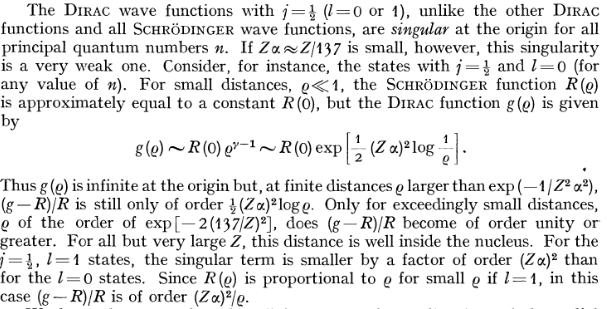
\includegraphics[width=\linewidth]{bethe-salpeter-QM-DiracDiv.png}
			\caption{QM by Bethe \& Salpeter}
			\label{fig:bethe-salpeter-QM-DiracDiv}
		\end{figure}
		
	\end{itemize}

\end{frame}
\begin{frame}
	\frametitle{Motivation}

	
	\begin{itemize}
		\item \red{Universal behaviors} in Coulombic wave functions, \orange{near-the-origin} \green{divergence} in relativistic wave functions (i.e. Hydrogen atom, Taylor expanded): 
	\end{itemize}
	\begin{align*}
		R^{\textrm{Schr}}_{n0}(r) & \propto
		\begin{cases}
			\arraycolsep=1.4pt\def\arraystretch{1.5}
			\begin{array}{lrll}
				1-\red{\dfrac{r}{a_0}}+ & \frac{1}{2} \blue{\dfrac{r^2}{a_0^2}}   & +\cdots & (n=1) \\
				1-\red{\dfrac{r}{a_0}}+ & \frac{3}{8} \blue{\dfrac{r^2}{a_0^2}}   & +\cdots & (n=2) \\
				1-\red{\dfrac{r}{a_0}}+ & \frac{19}{54} \blue{\dfrac{r^2}{a_0^2}} & +\cdots & (n=3) \\
				1-\red{\dfrac{r}{a_0}}+ & \frac{11}{32} \blue{\dfrac{r^2}{a_0^2}} & +\cdots & (n=4) \\
			\end{array}
		\end{cases},\\
		\only<1>{R^{\textrm{KG}}_{n0}(r)   & \propto
		\begin{cases}
			\arraycolsep=1.4pt\def\arraystretch{1.5}
			\begin{array}{lrll}
				1 -\red{\dfrac{r}{a_0}}     + & \frac{1}{2} \blue{\dfrac{r^2}{a_0^2}}   & -\orange{Z^2\alpha^2 \log{\left(\dfrac{r}{a_0}\right)}}+\green{Z^2\alpha^2 \left(\dfrac{r}{a_0}\right)\log{\left(\dfrac{r}{a_0}\right)}}+\cdots & \hspace{-5pt} (n=1) \\
				1 -\red{\dfrac{r}{a_0}}     + & \frac{3}{8} \blue{\dfrac{r^2}{a_0^2}}   & -\orange{Z^2\alpha^2 \log{\left(\dfrac{r}{a_0}\right)}}+\green{Z^2\alpha^2 \left(\dfrac{r}{a_0}\right)\log{\left(\dfrac{r}{a_0}\right)}}+\cdots & \hspace{-5pt} (n=2) \\
				1 -\red{\dfrac{r}{a_0}}    +  & \frac{19}{54} \blue{\dfrac{r^2}{a_0^2}} & -\orange{Z^2\alpha^2 \log{\left(\dfrac{r}{a_0}\right)}}+\green{Z^2\alpha^2 \left(\dfrac{r}{a_0}\right)\log{\left(\dfrac{r}{a_0}\right)}}+\cdots & \hspace{-5pt} (n=3) \\
				1 -\red{\dfrac{r}{a_0}}   +   & \frac{11}{32} \blue{\dfrac{r^2}{a_0^2}} & -\orange{Z^2\alpha^2 \log{\left(\dfrac{r}{a_0}\right)}}+\green{Z^2\alpha^2 \left(\dfrac{r}{a_0}\right)\log{\left(\dfrac{r}{a_0}\right)}}+\cdots & \hspace{-5pt} (n=4) \\
			\end{array}
		\end{cases}}
		\only<2>{
			R^{\textrm{Dirac}}_{n0}  (r) &\propto
		\begin{cases}
			\arraycolsep=1.4pt\def\arraystretch{1.5}
			\begin{array}{lrllll}
				1-\red{\dfrac{r}{a_0}}+       & \frac{1}{2} \blue{\dfrac{r^2}{a_0^2}}   & -\purple{\bm{\dfrac{1}{2}}}\orange{Z^2\alpha^2 \log{\left(\dfrac{r}{a_0}\right)}} & +  \purple{\bm{\dfrac{1}{2}}}\green{Z^2\alpha^2 \left(\dfrac{r}{a_0}\right)\log{\left(\dfrac{r}{a_0}\right)}} & +\cdots & \hspace{-5pt}  (n=1) \\
				1 -\red{\dfrac{r}{a_0}}     + & \frac{3}{8} \blue{\dfrac{r^2}{a_0^2}}   & -\purple{\bm{\dfrac{1}{2}}}\orange{Z^2\alpha^2 \log{\left(\dfrac{r}{a_0}\right)}} & +  \purple{\bm{\dfrac{1}{2}}}\green{Z^2\alpha^2 \left(\dfrac{r}{a_0}\right)\log{\left(\dfrac{r}{a_0}\right)}} & +\cdots & \hspace{-5pt} (n=2)  \\
				1 -\red{\dfrac{r}{a_0}}    +  & \frac{19}{54} \blue{\dfrac{r^2}{a_0^2}} & -\purple{\bm{\dfrac{1}{2}}}\orange{Z^2\alpha^2 \log{\left(\dfrac{r}{a_0}\right)}} & +  \purple{\bm{\dfrac{1}{2}}}\green{Z^2\alpha^2 \left(\dfrac{r}{a_0}\right)\log{\left(\dfrac{r}{a_0}\right)}} & +\cdots & \hspace{-5pt} (n=3)  \\
				1 -\red{\dfrac{r}{a_0}}   +   & \frac{11}{32} \blue{\dfrac{r^2}{a_0^2}} & -\purple{\bm{\dfrac{1}{2}}}\orange{Z^2\alpha^2 \log{\left(\dfrac{r}{a_0}\right)}} & +  \purple{\bm{\dfrac{1}{2}}}\green{Z^2\alpha^2 \left(\dfrac{r}{a_0}\right)\log{\left(\dfrac{r}{a_0}\right)}} & +\cdots & \hspace{-5pt} (n=4)  \\
			\end{array}
		\end{cases}
		}
	\end{align*}

\end{frame}

\begin{frame}
	\frametitle{Question: }
	\large
	\begin{itemize}
		\item \red{\bf What caused the state-independent logarithmic divergences? }
		\item \purple{\bf Hint: 
		\begin{itemize}
			\purple{
				\item Logarithms from the wave functions appear at order-$\alpha^2$, 
				\item anomalous dimensions of NRQCD also appear at order-$\alpha_s^2$,
				\item Bethe-Salpeter wave function is defined as $\mel{0}{\psi}{\Psi}$ in QFT, state-independency implies operator properties
				}
		\end{itemize}}
		\item Treat the nucleus as an infinitely heavy field, similar to HQET
		\item Natural assumption: the QFT correspondence of Dirac equation is QED
		\item UV behavior of Dirac wave functions + operator behavior 
		\Rightarrow Operator product expansion (OPE)
	\end{itemize}

\end{frame}

\begin{frame}
	\frametitle{Failed Attempt: OPE \& QED}

	
	\begin{itemize}
		\item QED + heavy nucleus effective theory (HNET): 
		\begin{align}
			%------------------------------------
			{\mathcal L}_{\rm UV} = \bar{\Psi}(i\slashed{D}-m)\Psi +N^\dagger iD_0 N-\frac{1}{4}F_{\mu\nu}F^{\mu\nu},
			%------------------------------------
			\label{UV:atom:lagrangian}
			%------------------------------------
		\end{align}
		$\Psi$: QED electron field\\
		$N$: nucleus field\\
		$F$: photon field, only considering Coulomb potential
		\item Dirac wave function: 
			\begin{align}
				%------------------------------------
				\Psi_{njm}({\bf r}) \equiv \langle 0 \vert  \Psi({\bf r}) N(0) \vert n j m \rangle,
				%------------------------------------
				\label{Dirac:wf:nonlocal:matrix:element}
				%------------------------------------
			\end{align}
	\end{itemize}


\end{frame}

\begin{frame}
	\frametitle{Failed Attempt: OPE \& QED}

	\begin{itemize}
		\item Operator Product Expansion (OPE): The limit when product of local operators at different points approach each other.
				\begin{align}
					T\phi(x)\phi(0)\sim\sum_{\mathcal{O}}C_{\mathcal{O}}(x^{\mu})[\mathcal{O}(0)]_R
				\end{align}
		\item Expand $\Psi({\bf r}) N(0)$ with OPE: 
		\begin{block}{\large OPE relation in coordinate space (QED)}
			\begin{align*}
				\Psi({\bf r})N({\bf 0})=(1 +{Z \alpha  \over \pi} \ln r)\,[\Psi N]({\bf 0})+\cdots
				% \label{OPEME}
			\end{align*}
		\end{block}
		\item \red{\bf Logarithms at order-$\alpha$!}
		\item Why? 
		
		The UV behavior of QED does not reflect the UV behavior of Dirac wave function. 
	\end{itemize}


\end{frame}

\begin{frame}
	\frametitle{The scales of an atom}

	%\begin{figure}[!htb]
	%	\centering
		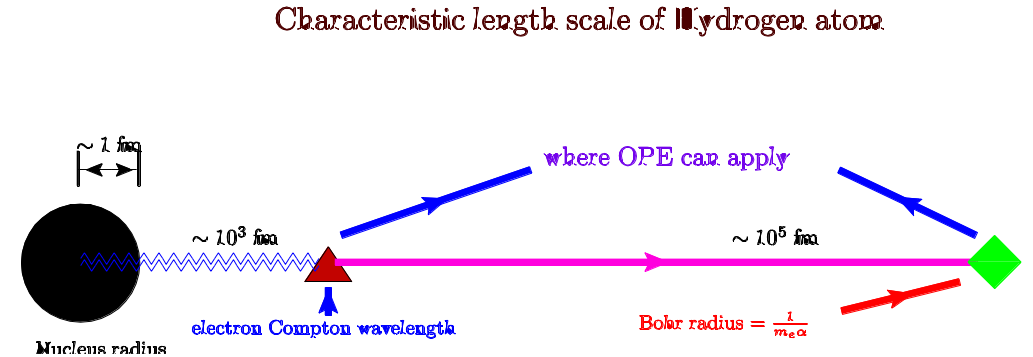
\includegraphics[width=\linewidth]{scale.png}
	%	\caption{}
	%	\label{fig:scale}
	%\end{figure}
	\begin{itemize}
		\item electron Compton wavelength is the IR scale of QED
		\item Desired OPE should probe the UV limit of an EFT whose effectiveness stays below $m_e$. 
	\end{itemize}

\end{frame}

\begin{frame}
	\frametitle{Attack the problem with OPE \& EFT: Construct EFT}

	
	\begin{itemize}
		\item Use \green{\bf non-relativistic QED (NRQED)} for electron and \purple{\bf heavy nucleus effective theory (HNET, similar to HQET)} for nucleus\only<2>{, \red{\bf keep only Coulomb potential}}. 
		\item Lagrangian for non-relativistic atoms:
		\begin{align}
			\mathcal{L}= \only<1>{{\cal L}_{\rm Max}}\only<2>{\bcancel{{\cal L}_{\rm Max}}\;\red{\mathcal{L}_{\rm Coul}}}+ {\cal L}_{\rm NRQED} +{\cal L}_{\rm HNET} + \delta {\cal L}_{\rm contact}
			\label{LAGFULL}
		\end{align}
		where
		\begin{align*}
			  & \only<1>{{\cal L}_{\rm Max}= -\frac{1}{4} d_\gamma F_{\mu\nu}F^{\mu\nu}+\cdots, }\only<2>{\red{{\cal L}_{\rm Coul}= 
			  \frac{1}{2} \left(\nabla A^0\right)^2}},                             \\
			  & {\cal L}_{\rm NRQED}={\psi^\dagger \Bigg\{\red{iD_0+ {{\bf D}^2 \over 2m}} + \orange{ {{\bf D}^4\over 8m^3}+c_D e
			  {[\bm\nabla\cdot {\bf E}]\over 8m^2}}+\cdots\Bigg\}},\\
			%   c_D e
				% {[\bm\nabla\cdot {\bf E}]\over 8m^2}+c_F e {{\bm\sigma}\cdot{\bf B}\over 2m}+ ic_S e {({\bf D}\times {\bf E}-{\bf E}\times {\bf D})\cdot
			% \bm{\sigma}\over 8m^2}+\cdots\Bigg\}\psi,}\\
			  & {\cal L}_{\rm HNET}= \red{N^\dagger i D_0 N}+\cdots,                                                     \\
			  & \only<1>{\delta {\cal L}_{\rm contact}= {c_4\over m^2} \psi^\dagger\psi N^\dagger N+\cdots,}\only<2>{\xcancel{\delta {\cal L}_{\rm contact}= {c_4\over m^2} \psi^\dagger\psi N^\dagger N+\cdots,}}
		\end{align*}
		where $D^\mu=\partial^\mu+ieA^\mu$.
	\end{itemize}

\end{frame}

\begin{frame}
	\frametitle{Attack the problem with OPE \& EFT: Renormalization of the local operator}

	
	\begin{itemize}
		\item Use 4-point Green function as testing ground. 
		\item The renormalization constant of $[\psi N](0)$: 
		\begin{align}
			\bqty{\psi N}_R=Z_\mathcal{S}{\psi N}
		\end{align}
		\item The total divergence coming from the local operator (MS scheme)
		\begin{align}
			%------------------------------------
			Z_{\mathcal{S}}=1-\frac{Z^2\alpha^2}{4\epsilon}+\cdots.
			%------------------------------------
			\label{compo-renorm}
			%------------------------------------
		\end{align}
			%------------------------------------
		\item The anomalous dimension of the operator $\psi N$ then reads
			%------------------------------------
		\begin{align}
			%------------------------------------
			\gamma_{\mathcal{S}}\equiv {d\ln Z_\mathcal{S} \over d\ln\mu}= {Z^2\alpha^2\over 2}.
			%------------------------------------
			\label{ano-dim}
			%------------------------------------
		\end{align}
	\end{itemize}

\end{frame}

\begin{frame}
	\frametitle{Attack the problem with OPE \& EFT: Renormalization of local operators}

	\begin{figure}[!hbtp]
		\centering
		\begin{tabular}{ccccc}
			  & \null\hfill
			\subfloat[\red{\checkmark}]{
				$$\begin{tikzpicture}[baseline=($(p1)!0.5!(x)$)]
						\begin{feynman}
							\vertex (p1);
							\vertex[right=1.7cm of p1] (p2);
							\node[crossed dot] at ($(p1)!0.5!(p2)+(0,2cm)$) (x) ;
							\vertex at ($(p1)!0.2!(x)$) (y1);
							\vertex at ($(p2)!0.2!(x)$) (z1);
							\vertex at ($(p1)!0.6!(x)$) (y2);
							\vertex at ($(p2)!0.6!(x)$) (z2);
							\vertex at ($(y1)!0.5!(z1)$) (t);
							%
							\diagram* {
							(y1) -- [scalar] (z1);
							(y2) -- [scalar] (z2);
							(p1) -- [fermion] (y1);
							(p2) -- [HQET] (z1);
							(y1) -- [insertion={[style=thick,size=3pt]0.7},with arrow=0.4] (y2);
							(z1) -- [HQET] (z2);
							(y2) -- [fermion] (x);
							(z2) -- [HQET] (x);
							};
						\end{feynman}
					\end{tikzpicture}$$
			}\hfill
			  & \subfloat[]{
				$$\begin{tikzpicture}[baseline=($(p1)!0.5!(x)$)]
						\begin{feynman}
							\vertex (p1);
							\vertex[right=1.7cm of p1] (p2);
							\node[crossed dot] at ($(p1)!0.5!(p2)+(0,2cm)$) (x) ;
							\vertex at ($(p1)!0.2!(x)$) (y1);
							\vertex at ($(p2)!0.2!(x)$) (z1);
							\vertex at ($(p1)!0.6!(x)$) (y2);
							\vertex at ($(p2)!0.6!(x)$) (z2);
							\vertex at ($(y1)!0.5!(z1)$) (t);
							%
							\diagram* {
							(y1) -- [scalar] (z1);
							(y2) -- [scalar] (z2);
							(p1) -- [fermion] (y1);
							(p2) -- [HQET] (z1);
							(y1) -- [fermion] (y2);
							(z1) -- [HQET] (z2);
							(y2) -- [insertion={[style=thick,size=3pt]0.7},with arrow=0.4] (x);
							(z2) -- [HQET] (x);
							};
						\end{feynman}
					\end{tikzpicture}$$
			}
			\hfill
			  & \subfloat[\red{\checkmark}]{
				$$\begin{tikzpicture}[baseline=($(p1)!0.5!(x)$)]
						\begin{feynman}
							\vertex (p1);
							\vertex[right=1.7cm of p1] (p2);
							\node[crossed dot] at ($(p1)!0.5!(p2)+(0,2cm)$) (x) ;
							\vertex at ($(p1)!0.2!(x)$) (y1);
							\node [square dot,minimum size=1.3mm] at ($(y1)$) (tmp);
							\vertex at ($(p2)!0.2!(x)$) (z1);
							\vertex at ($(p1)!0.6!(x)$) (y2);
							\vertex at ($(p2)!0.6!(x)$) (z2);
							%
							\diagram* {
							(y1) -- [scalar] (z1);
							(y2) -- [scalar] (z2);
							(p1) -- [fermion] (y1);
							(p2) -- [HQET] (z1);
							(y1) -- [fermion] (y2);
							(z1) -- [HQET] (z2);
							(y2) -- [fermion] (x);
							(z2) -- [HQET] (x);
							};
						\end{feynman}
					\end{tikzpicture}$$
			}
			\hfill
			  & \subfloat[]{
				$$\begin{tikzpicture}[baseline=($(p1)!0.5!(x)$)]
						\begin{feynman}
							\vertex (p1);
							\vertex[right=1.7cm of p1] (p2);
							\node[crossed dot] at ($(p1)!0.5!(p2)+(0,2cm)$) (x) ;
							\vertex at ($(p1)!0.2!(x)$) (y1);
							\vertex at ($(p2)!0.2!(x)$) (z1);
							\vertex at ($(p1)!0.6!(x)$) (y2);
							\node [square dot,minimum size=1.3mm] at ($(y2)$) (tmp);
							\vertex at ($(p2)!0.6!(x)$) (z2);
							%
							\diagram* {
							% (y1) -- [scalar,rmomentum'={[arrow style=white]$l_1$},white] (z1);
							(y1) -- [scalar] (z1);
							(y2) -- [scalar] (z2);
							(p1) -- [fermion] (y1);
							(p2) -- [HQET] (z1);
							(y1) -- [fermion] (y2);
							(z1) -- [HQET] (z2);
							(y2) -- [fermion] (x);
							(z2) -- [HQET] (x);
							};
						\end{feynman}
					\end{tikzpicture}$$
			}\\
			  & \null\hfill
			\subfloat[]{
				$$\begin{tikzpicture}[baseline=($(p1)!0.5!(x)$),remember picture]
						\begin{feynman}
							\vertex (p1);
							\vertex[right=1.7cm of p1] (p2);
							\node[crossed dot] at ($(p1)!0.5!(p2)+(0,2cm)$) (x) ;
							\vertex at ($(p1)!0.2!(x)$) (y1);
							\vertex at ($(p2)!0.2!(x)$) (z1);
							\vertex at ($(p1)!0.6!(x)$) (y2);
							\vertex at ($(p2)!0.6!(x)$) (z2);
							%
							\diagram* {
							(y1) -- [scalar] (z1);
							(y2) -- [scalar] (z2);
							(p1) -- [fermion] (y1);
							(p2) -- [HQET] (z1);
							(y1) -- [fermion] (y2);
							(z1) -- [HQET] (z2);
							(y2) -- [fermion] (x);
							(z2) -- [HQET] (x);
							};
							\node [square dot] at ($(y1)$) (tmp);
							\node [empty square dot] at ($(y1)$) (tmp1);
						\end{feynman}
					\end{tikzpicture}$$
				\label{subfig:SO1}
			}\hfill
			  & \subfloat[]{
				$$\begin{tikzpicture}[baseline=($(p1)!0.5!(x)$),remember picture]
						\begin{feynman}
							\vertex (p1);
							\vertex[right=1.7cm of p1] (p2);
							\node[crossed dot] at ($(p1)!0.5!(p2)+(0,2cm)$) (x) ;
							\vertex at ($(p1)!0.2!(x)$) (y1);
							\vertex at ($(p2)!0.2!(x)$) (z1);
							\vertex at ($(p1)!0.6!(x)$) (y2);
							\vertex at ($(p2)!0.6!(x)$) (z2);
							%
							\diagram* {
							(y1) -- [scalar] (z1);
							(y2) -- [scalar] (z2);
							(p1) -- [fermion] (y1);
							(p2) -- [HQET] (z1);
							(y1) -- [fermion] (y2);
							(z1) -- [HQET] (z2);
							(y2) -- [fermion] (x);
							(z2) -- [HQET] (x);
							};
							\node [square dot] at ($(y2)$) (tmp);
							\node [empty square dot] at ($(y2)$) (tmp1);
						\end{feynman}
					\end{tikzpicture}$$
				\label{subfig:SO2}
			}\hfill
			& \subfloat[]{
				\begin{tikzpicture}[baseline=($(p1)!0.5!(x)$)]
					\begin{feynman}
						\vertex (p1);
						\vertex[right=1.7cm of p1] (p2);
						\node[crossed dot] at ($(p1)!0.5!(p2)+(0,2cm)$) (x) ;
						% \vertex[above=2cm of p1] (x)  ;
						% \vertex[above=2cm of p2] (0)  ;
						\vertex at ($(p1)!0.5!(p2)$) (p0) ;
						\node[empty dot] at ($(p0)!0.4!(x)$) (i);
						\vertex at ($(p0)!0.66!(x)+(0.85cm,0)$) (y1);
						\vertex[right=2.2cm of y1] (z1);
						% \vertex[above=0.05cm of x] (text) {\(0\)};
						%
						\diagram* {
						(p1) -- [fermion] (i);
						(p2) -- [HQET] (i);
						(i) -- [fermion,half left] (x);
						% (y1) -- [] (x);
						(i) -- [HQET, half right] (x);
						%(z1) -- [double distance=1pt] (0);
						%(y1) -- [photon] (z1);
						};
					\end{feynman}
				\end{tikzpicture}
			}\hfill
			& \subfloat[]{
				\begin{tikzpicture}[baseline=($(p1)!0.5!(x)$)]
					\begin{feynman}
						\vertex (p1);
						\vertex[right=1.7cm of p1] (p2);
						\node[crossed dot] at ($(p1)!0.5!(p2)+(0,2cm)$) (x) ;
						% \vertex[above=2cm of p1] (x)  ;
						% \vertex[above=2cm of p2] (0)  ;
						\vertex at ($(p1)!0.5!(p2)$) (p0) ;
						\node[empty dot] at ($(p0)!0.4!(x)$) (i);
						\vertex at ($(p0)!0.66!(x)+(-0.65cm,0)$) (y1);
						\vertex at ($(p0)!0.66!(x)+(0.65cm,0)$) (z1);
						% \vertex[above=0.05cm of x] (text) {\(0\)};
						%
						\diagram* {
						(p1) -- [fermion] (i);
						(p2) -- [double distance=1pt] (i);
						(i) -- [fermion,quarter left] (y1);
						(y1) -- [fermion, quarter left] (x);
						(i) -- [HQET, quarter right] (z1);
						(z1) -- [HQET,quarter right] (x);
						(y1) -- [scalar] (z1);
						};
					\end{feynman}
				\end{tikzpicture}
			}
	\end{tabular}
	\caption{\label{Fig:vertex:corr:all} Representative diagrams for local operator renormalization. The cap represents the
	insertion of the operator $\psi N$, cross stands for the ${\bf p}^4$ relativistic correction,
	solid square for the Darwin vertex, while empty square for spin-orbital vertex, which making vanishing contribution
	in this case. The empty circle represents the contact interaction.
	The last two diagrams are beyond the prescribed accuracy of ${\cal O}(Z^2\alpha^2)$.}
	\end{figure}

\end{frame}



\begin{frame}
	\frametitle{Attack the problem with OPE \& EFT: Wilson coefficients}

	\newcommand{\scalefactor}{0.75}
	\begin{figure}[pbth]
		\centering
		\begin{displaymath}\begin{split}&\hspace{-2mm}
		\begin{tikzpicture}[baseline=($(p1)!0.5!(x)$),transform shape,scale=\scalefactor]
			\begin{feynman}
				\vertex (p1);
				\vertex[right=1.2cm of p1] (p2);
				\vertex at ($(p1)!0.3!(p2)+(0,1.8cm)$) (x) {\(\vb{r}\)};
				\vertex at ($(p1)!0.7!(p2)+(0,1.8cm)$) (0) {\(\vb{0}\)};
				\vertex at ($(p1)!0.35!(x)$) (y1);
				\vertex at ($(p2)!0.35!(0)$) (z1);
				%
				\diagram* {
				(y1) -- [scalar] (z1);
				(p1) -- [fermion,edge label=\(p\)] (y1);
				(p2) -- [HQET,momentum'=\(k\)] (z1);
				(y1) -- [fermion,edge label=\(\vb{q}\)] (x);
				(z1) -- [HQET] (0);
				};
			\end{feynman}
		\end{tikzpicture}=
		\pqty{\begin{tikzpicture}[baseline=($(p1)!0.5!(x2)$),transform shape,scale=\scalefactor]
			\begin{feynman}
				\vertex                  (p1) ;
				\vertex[right=1.2cm of p1] (p2) ;
				\vertex at ($(p1)!0.3!(p2)+(0,1.8cm)$) (x2) {\(\vb{r}\)};
				\vertex at ($(p1)!0.7!(p2)+(0,1.8cm)$) (02) {\(\vb{0}\)};
				\node[crossed dot,minimum size=\dotsize] at ($(p1)!0.5!(p2)+(0,0.65cm)$) (x) ;
				\vertex at ($(p1)!0.1!(x2)$) (p12);
				\vertex[right=1.2cm of p12] (p22);
				\vertex at ($(p12)!0.5!(x2)$) (y12);
				\vertex at ($(p22)!0.5!(02)$) (z12);
				%
				\diagram* {
					(p1) -- [fermion,edge label=\(p\)] (x);
					(p2) -- [HQET,momentum'=\(k\)] (x);
				};
				\diagram* {
				(y12) -- [very thick, scalar] (z12);
				(y12) -- [very thick,fermion,edge label=\(\vb{q}\)] (x2);
				(z12) -- [very thick, HQET] (02);
				};
				% \vertex at ($(x2)!1.4!(y12)$) (tail1);
				% \vertex at ($(02)!1.4!(z12)$) (tail2);
				% \diagram*{
				% 	(tail1) -- [fermion] (y12);
				% 	(tail2) -- [HQET] (z12);
				% };
			\end{feynman}
		\end{tikzpicture}-\begin{tikzpicture}[baseline=($(p1)!0.5!(x)$),transform shape,scale=\scalefactor]
			\begin{feynman}
				\vertex (p1);
				\vertex[right=1.2cm of p1] (p2);
				\node[crossed dot,minimum size=\dotsize] at ($(p1)!0.5!(p2)+(0,1.8cm)$) (x) ;
				\vertex at ($(p1)!0.35!(x)$) (y1);
				\vertex at ($(p2)!0.35!(x)$) (z1);
				%
				\diagram* {
				(y1) -- [very thick,scalar] (z1);
				(p1) -- [fermion,edge label=\(p\)] (y1);
				(p2) -- [HQET,momentum'=\(k\)] (z1);
				(y1) -- [very thick,fermion] (x);
				(z1) -- [very thick,HQET] (x);
				};
			\end{feynman}
		\end{tikzpicture}-\text{UVCT}}%\\&
		+\pqty{
		\begin{tikzpicture}[baseline=($(p1)!0.5!(x)$),transform shape,scale=\scalefactor]
			\begin{feynman}
				\vertex (p1);
				\vertex[right=1.2cm of p1] (p2);
				\node[crossed dot,minimum size=\dotsize] at ($(p1)!0.5!(p2)+(0,1.8cm)$) (x) ;
				\vertex at ($(p1)!0.35!(x)$) (y1);
				\vertex at ($(p2)!0.35!(x)$) (z1);
				%
				\diagram* {
				(y1) -- [scalar] (z1);
				(p1) -- [fermion,edge label=\(p\)] (y1);
				(p2) -- [HQET,momentum'=\(k\)] (z1);
				(y1) -- [fermion] (x);
				(z1) -- [HQET] (x);
				};
			\end{feynman}
		\end{tikzpicture}+\text{UVCT}}\\&
		\begin{tikzpicture}[baseline=($(p1)!0.5!(x)$),transform shape,scale=\scalefactor]
			\begin{feynman}
				\vertex (p1);
				\vertex[right=1.2cm of p1] (p2);
				\vertex at ($(p1)!0.3!(p2)+(0,1.8cm)$) (x) {\(\vb{r}\)};
				\vertex at ($(p1)!0.7!(p2)+(0,1.8cm)$) (0) {\(\vb{0}\)};
				\vertex at ($(p1)!0.2!(x)$) (y1);
				\vertex at ($(p2)!0.2!(0)$) (z1);
				\vertex at ($(p1)!0.7!(x)$) (y2);
				\vertex at ($(p2)!0.7!(0)$) (z2);
				%
				\diagram* {
				(y1) -- [scalar] (z1);
				(y2) -- [scalar] (z2);
				(p1) -- [fermion] (y1);
				(p2) -- [HQET] (z1);
				(y1) -- [with arrow=0.4,insertion={[style=thick,size=3pt]0.7}] (y2);
				(z1) -- [HQET] (z2);
				(y2) -- [fermion] (x);
				(z2) -- [HQET] (0);
				};
			\end{feynman}
		\end{tikzpicture}=
		\pqty{\begin{tikzpicture}[baseline=($(p1)!0.5!(x2)$),transform shape,scale=\scalefactor]
			\begin{feynman}
				\vertex                  (p1) ;
				\vertex[right=1.2cm of p1] (p2) ;
				\node[crossed dot,minimum size=\dotsize] at ($(p1)!0.5!(p2)+(0,0.4cm)$) (x) ;
				\vertex[above=0.4cm of p1] (p12);
				\vertex[right=1.2cm of p12] (p22);
				\vertex at ($(p12)!0.3!(p22)+(0,1.4cm)$) (x2) {\(\vb{r}\)};
				\vertex at ($(p12)!0.7!(p22)+(0,1.4cm)$) (02) {\(\vb{0}\)};
				\vertex at ($(p12)!0.2!(x2)$) (y12);
				\vertex at ($(p22)!0.2!(02)$) (z12);
				\vertex at ($(p12)!0.6!(x2)$) (y22);
				\vertex at ($(p22)!0.6!(02)$) (z22);
				%
				\diagram* {
				(p1) -- [fermion] (x);
				(p2) -- [HQET] (x);
				};
				\diagram* {
				(y12) -- [very thick, scalar] (z12);
				(y22) -- [very thick, scalar] (z22);
				(y12) -- [very thick,with arrow=0.4,insertion={[style=thick,size=3pt]0.7}] (y22);
				(z12) -- [very thick, HQET] (z22);
				(y22) -- [very thick,fermion] (x2);
				(z22) -- [very thick, HQET] (02);
				};
				% \vertex at ($(x2)!1.3!(y12)$) (tail1);
				% \vertex at ($(02)!1.3!(z12)$) (tail2);
				% \diagram*{
				% 	(tail1) -- [fermion] (y12);
				% 	(tail2) -- [HQET] (z12);
				% };
			\end{feynman}
		\end{tikzpicture}-\begin{tikzpicture}[baseline=($(p1)!0.5!(x)$),transform shape,scale=\scalefactor]
			\begin{feynman}
				\vertex (p1);
				\vertex[right=1.2cm of p1] (p2);
				\node[crossed dot,minimum size=\dotsize] at ($(p1)!0.5!(p2)+(0,1.8cm)$) (x) ;
				\vertex at ($(p1)!0.2!(x)$) (y1);
				\vertex at ($(p2)!0.2!(x)$) (z1);
				\vertex at ($(p1)!0.6!(x)$) (y2);
				\vertex at ($(p2)!0.6!(x)$) (z2);
				\vertex at ($(y1)!0.5!(z1)$) (t);
				%
				\diagram* {
				(y1) -- [very thick,scalar] (z1);
				(y2) -- [very thick,scalar] (z2);
				(p1) -- [fermion] (y1);
				(p2) -- [HQET] (z1);
				(y1) -- [very thick,with arrow=0.4,insertion={[style=thick,size=3pt]0.7}] (y2);
				(z1) -- [very thick,HQET] (z2);
				(y2) -- [very thick,fermion] (x);
				(z2) -- [very thick,HQET] (x);
				};
			\end{feynman}
		\end{tikzpicture}-\text{UVCT}}%\\&\hspace{-0.6in}
		+\pqty{\begin{tikzpicture}[baseline=($(p1)!0.5!(x2)$),transform shape,scale=\scalefactor]
			\begin{feynman}
				\vertex                  (p1) ;
				\vertex[right=1.2cm of p1] (p2) ;
				\node[crossed dot,minimum size=\dotsize] at ($(p1)!0.5!(p2)+(0,1cm)$) (x) ;
				\vertex at ($(p1)!0.3!(x)$) (y1);
				\vertex at ($(p2)!0.3!(x)$) (z1);
				\vertex[above=1cm of p1] (p12);
				\vertex[right=1.2cm of p12] (p22);
				\vertex at ($(p12)!0.3!(p22)+(0,0.8cm)$) (x2) {\(\vb{r}\)};
				\vertex at ($(p12)!0.7!(p22)+(0,0.8cm)$) (02) {\(\vb{0}\)};
				\vertex at ($(p12)!0.4!(x2)$) (y12);
				\vertex at ($(p22)!0.4!(02)$) (z12);
				%
				\diagram* {
					(y1) -- [scalar] (z1);
					(p1) -- [fermion] (y1);
					(p2) -- [HQET] (z1);
					(y1) -- [with arrow=0.4,insertion={[style=thick,size=3pt]0.7}] (x);
					(z1) -- [HQET] (x);
				};
				\diagram* {
				(y12) -- [very thick, scalar] (z12);
				(y12) -- [very thick,fermion] (x2);
				(z12) -- [very thick, HQET] (02);
				};
				% \vertex at ($(x2)!1.6!(y12)$) (tail1);
				% \vertex at ($(02)!1.6!(z12)$) (tail2);
				% \diagram*{
				% 	(tail1) -- [fermion] (y12);
				% 	(tail2) -- [HQET] (z12);
				% };
			\end{feynman}
		\end{tikzpicture}-\begin{tikzpicture}[baseline=($(p1)!0.5!(x)$),transform shape,scale=\scalefactor]
			\begin{feynman}
				\vertex (p1);
				\vertex[right=1.2cm of p1] (p2);
				\node[crossed dot,minimum size=\dotsize] at ($(p1)!0.5!(p2)+(0,1.8cm)$) (x) ;
				\vertex at ($(p1)!0.2!(x)$) (y1);
				\vertex at ($(p2)!0.2!(x)$) (z1);
				\vertex at ($(p1)!0.6!(x)$) (y2);
				\vertex at ($(p2)!0.6!(x)$) (z2);
				\vertex at ($(y1)!0.5!(z1)$) (t);
				%
				\diagram* {
				(y1) -- [scalar] (z1);
				(y2) -- [very thick,scalar] (z2);
				(p1) -- [fermion] (y1);
				(p2) -- [HQET] (z1);
				(y1) -- [with arrow=0.4,insertion={[style=thick,size=3pt]0.7}] (y2);
				(z1) -- [HQET] (z2);
				(y2) -- [very thick,fermion] (x);
				(z2) -- [very thick,HQET] (x);
				};
			\end{feynman}
		\end{tikzpicture}}+
		\pqty{\begin{tikzpicture}[baseline=($(p1)!0.5!(x)$),transform shape,scale=\scalefactor]
			\begin{feynman}
				\vertex (p1);
				\vertex[right=1.2cm of p1] (p2);
				\node[crossed dot,minimum size=\dotsize] at ($(p1)!0.5!(p2)+(0,1.8cm)$) (x) ;
				\vertex at ($(p1)!0.2!(x)$) (y1);
				\vertex at ($(p2)!0.2!(x)$) (z1);
				\vertex at ($(p1)!0.6!(x)$) (y2);
				\vertex at ($(p2)!0.6!(x)$) (z2);
				\vertex at ($(y1)!0.5!(z1)$) (t);
				%
				\diagram* {
				(y1) -- [scalar] (z1);
				(y2) -- [scalar] (z2);
				(p1) -- [fermion] (y1);
				(p2) -- [HQET] (z1);
				(y1) -- [with arrow=0.4,insertion={[style=thick,size=3pt]0.7}] (y2);
				(z1) -- [HQET] (z2);
				(y2) -- [fermion] (x);
				(z2) -- [HQET] (x);
				};
			\end{feynman}
		\end{tikzpicture}+\text{UVCT}}\\&
		\begin{tikzpicture}[baseline=($(p1)!0.5!(x)$),transform shape,scale=\scalefactor]
			\begin{feynman}
				\vertex (p1);
				\vertex[right=1.2cm of p1] (p2);
				\vertex at ($(p1)!0.3!(p2)+(0,1.8cm)$) (x) {\(\vb{r}\)};
				\vertex at ($(p1)!0.7!(p2)+(0,1.8cm)$) (0) {\(\vb{0}\)};
				\node[square dot] at ($(p1)!0.2!(x)$) (y1);
				\vertex at ($(p2)!0.2!(0)$) (z1);
				\vertex at ($(p1)!0.7!(x)$) (y2);
				\vertex at ($(p2)!0.7!(0)$) (z2);
				%
				\diagram* {
				(y1) -- [scalar] (z1);
				(y2) -- [scalar] (z2);
				(p1) -- [fermion] (y1);
				(p2) -- [HQET] (z1);
				(y1) -- [fermion] (y2);
				(z1) -- [HQET] (z2);
				(y2) -- [fermion] (x);
				(z2) -- [HQET] (0);
				};
			\end{feynman}
		\end{tikzpicture}=
		\pqty{\begin{tikzpicture}[baseline=($(p1)!0.5!(x2)$),transform shape,scale=\scalefactor]
			\begin{feynman}
				\vertex                  (p1) ;
				\vertex[right=1.2cm of p1] (p2) ;
				\node[crossed dot,minimum size=\dotsize] at ($(p1)!0.5!(p2)+(0,0.4cm)$) (x) ;
				\vertex[above=0.4cm of p1] (p12);
				\vertex[right=1.2cm of p12] (p22);
				\vertex at ($(p12)!0.3!(p22)+(0,1.4cm)$) (x2) {\(\vb{r}\)};
				\vertex at ($(p12)!0.7!(p22)+(0,1.4cm)$) (02) {\(\vb{0}\)};
				\node[square dot] at ($(p12)!0.2!(x2)$) (y12);
				\vertex at ($(p22)!0.2!(02)$) (z12);
				\vertex at ($(p12)!0.6!(x2)$) (y22);
				\vertex at ($(p22)!0.6!(02)$) (z22);
				%
				\diagram* {
				(p1) -- [fermion] (x);
				(p2) -- [HQET] (x);
				};
				\diagram* {
				(y12) -- [very thick, scalar] (z12);
				(y22) -- [very thick, scalar] (z22);
				(y12) -- [very thick,fermion] (y22);
				(z12) -- [very thick, HQET] (z22);
				(y22) -- [very thick,fermion] (x2);
				(z22) -- [very thick, HQET] (02);
				};
				% \vertex at ($(x2)!1.3!(y12)$) (tail1);
				% \vertex at ($(02)!1.3!(z12)$) (tail2);
				% \diagram*{
				% 	(tail1) -- [fermion] (y12);
				% 	(tail2) -- [HQET] (z12);
				% };
			\end{feynman}
		\end{tikzpicture}-\begin{tikzpicture}[baseline=($(p1)!0.5!(x)$),transform shape,scale=\scalefactor]
			\begin{feynman}
				\vertex (p1);
				\vertex[right=1.2cm of p1] (p2);
				\node[crossed dot,minimum size=\dotsize] at ($(p1)!0.5!(p2)+(0,1.8cm)$) (x) ;
				\node[square dot] at ($(p1)!0.2!(x)$) (y1);
				\vertex at ($(p2)!0.2!(x)$) (z1);
				\vertex at ($(p1)!0.6!(x)$) (y2);
				\vertex at ($(p2)!0.6!(x)$) (z2);
				\vertex at ($(y1)!0.5!(z1)$) (t);
				%
				\diagram* {
				(y1) -- [very thick,scalar] (z1);
				(y2) -- [very thick,scalar] (z2);
				(p1) -- [fermion] (y1);
				(p2) -- [HQET] (z1);
				(y1) -- [very thick,fermion] (y2);
				(z1) -- [very thick,HQET] (z2);
				(y2) -- [very thick,fermion] (x);
				(z2) -- [very thick,HQET] (x);
				};
			\end{feynman}
		\end{tikzpicture}-\text{UVCT}}%\\&\hspace{-0.6in}
		+\pqty{\begin{tikzpicture}[baseline=($(p1)!0.5!(x2)$),transform shape,scale=\scalefactor]
			\begin{feynman}
				\vertex                  (p1) ;
				\vertex[right=1.2cm of p1] (p2) ;
				\node[crossed dot,minimum size=\dotsize] at ($(p1)!0.5!(p2)+(0,1cm)$) (x) ;
				\node[square dot] at ($(p1)!0.3!(x)$) (y1);
				\vertex at ($(p2)!0.3!(x)$) (z1);
				\vertex[above=1cm of p1] (p12);
				\vertex[right=1.2cm of p12] (p22);
				\vertex at ($(p12)!0.3!(p22)+(0,0.8cm)$) (x2) {\(\vb{r}\)};
				\vertex at ($(p12)!0.7!(p22)+(0,0.8cm)$) (02) {\(\vb{0}\)};
				\vertex at ($(p12)!0.4!(x2)$) (y12);
				\vertex at ($(p22)!0.4!(02)$) (z12);
				%
				\diagram* {
					(y1) -- [scalar] (z1);
					(p1) -- [fermion] (y1);
					(p2) -- [HQET] (z1);
					(y1) -- [fermion] (x);
					(z1) -- [HQET] (x);
				};
				\diagram* {
				(y12) -- [very thick, scalar] (z12);
				(y12) -- [very thick,fermion] (x2);
				(z12) -- [very thick, HQET] (02);
				};
				% \vertex at ($(x2)!1.6!(y12)$) (tail1);
				% \vertex at ($(02)!1.6!(z12)$) (tail2);
				% \diagram*{
				% 	(tail1) -- [fermion] (y12);
				% 	(tail2) -- [HQET] (z12);
				% };
			\end{feynman}
		\end{tikzpicture}-\begin{tikzpicture}[baseline=($(p1)!0.5!(x)$),transform shape,scale=\scalefactor]
			\begin{feynman}
				\vertex (p1);
				\vertex[right=1.2cm of p1] (p2);
				\node[crossed dot,minimum size=\dotsize] at ($(p1)!0.5!(p2)+(0,1.8cm)$) (x) ;
				\node[square dot] at ($(p1)!0.2!(x)$) (y1);
				\vertex at ($(p2)!0.2!(x)$) (z1);
				\vertex at ($(p1)!0.6!(x)$) (y2);
				\vertex at ($(p2)!0.6!(x)$) (z2);
				\vertex at ($(y1)!0.5!(z1)$) (t);
				%
				\diagram* {
				(y1) -- [scalar] (z1);
				(y2) -- [very thick,scalar] (z2);
				(p1) -- [fermion] (y1);
				(p2) -- [HQET] (z1);
				(y1) -- [fermion] (y2);
				(z1) -- [HQET] (z2);
				(y2) -- [very thick,fermion] (x);
				(z2) -- [very thick,HQET] (x);
				};
			\end{feynman}
		\end{tikzpicture}}+
		\pqty{\begin{tikzpicture}[baseline=($(p1)!0.5!(x)$),transform shape,scale=\scalefactor]
			\begin{feynman}
				\vertex (p1);
				\vertex[right=1.2cm of p1] (p2);
				\node[crossed dot,minimum size=\dotsize] at ($(p1)!0.5!(p2)+(0,1.8cm)$) (x) ;
				\node[square dot] at ($(p1)!0.2!(x)$) (y1);
				\vertex at ($(p2)!0.2!(x)$) (z1);
				\vertex at ($(p1)!0.6!(x)$) (y2);
				\vertex at ($(p2)!0.6!(x)$) (z2);
				\vertex at ($(y1)!0.5!(z1)$) (t);
				%
				\diagram* {
				(y1) -- [scalar] (z1);
				(y2) -- [scalar] (z2);
				(p1) -- [fermion] (y1);
				(p2) -- [HQET] (z1);
				(y1) -- [fermion] (y2);
				(z1) -- [HQET] (z2);
				(y2) -- [fermion] (x);
				(z2) -- [HQET] (x);
				};
			\end{feynman}
		\end{tikzpicture}+\text{UVCT}}
		\end{split}\end{displaymath}
		\caption{Illustration of the OPE structure of the four-point Green functions through order
	$Z^2\alpha^2$. The first line is for the Wilson coefficient ${\cal C}^{(1)}(r)$,
	the two bottom lines for the Wilson coefficient ${\cal C}^{(2)}(r)$.
	The thick line indicates the corresponding loop momentum to be ``hard'' $(\sim {\bf q})$.}
	\label{Wilson:coeff:coor:space:decomp}
	\end{figure}

\end{frame}

\begin{frame}
	\frametitle{Attack the problem with OPE \& EFT: OPE}

	
	\onslide<+->\metroset{block=fill}
	\begin{block}{\large Correct OPE relation in coordinate space}
		\begin{align*}
			\psi({\bf r})N({\bf 0}) =\bqty{1- mZ\alpha r -{Z^2\alpha^2\over 2} \left(\ln \mu r+{\rm const} \right)
			+{\cal O}(Z^3\alpha^3)}\,[\psi N]({\bf 0})+\cdots
			% \label{OPEME}
		\end{align*}
	\end{block}

	\begin{block}{\large Correct OPE relation in momentum space}
		\begin{align*}
			\widetilde\psi({\bf q})N({\bf 0}) & \equiv \int d^3 {\bf r}
			e^{-i {\bf q}\cdot {\bf r}} \psi({\bf r})N({\bf 0})\nonumber\\&= 
			\bqty{{8\pi mZ\alpha+{\cal O}(Z^3\alpha^3) \over \abs{\bf q}^4}
			- {\pi^2 Z^2\alpha^2+{\cal O}(Z^4\alpha^4) \over |{\bf q}|^3}} [\psi N]({\bf 0})+\cdots.
			% \label{OPEMEMOM}
		\end{align*}
	\end{block}
	\begin{itemize}
		\item $\log r$ behavior is the same with the Dirac wave function. 
	\end{itemize}
\end{frame}

\begin{frame}
	\frametitle{Attack the problem with OPE \& EFT: Resumming logarithms with RGE} 

	\begin{itemize}
		\item The l.h.s. of the OPE relation is scale independent.
		\item We can write down the renormalization group equation of the Wilson coefficient: 
		\begin{align}
			%------------------------------------
			\mu {\partial {\cal C}(r,\mu)\over \partial \mu}+  \gamma_{\mathcal S} {\cal C}(r,\mu) = 0,
			%------------------------------------
			\label{RGE:cal:C:r:mu}
			%------------------------------------
		\end{align}
		\item Dimensional analysis leads to 
		\begin{align}
			%------------------------------------
			r {\partial {\cal C} \over \partial r}+ \gamma_{\mathcal S} {\cal C} = 0.
			%------------------------------------
			\label{RGE:cal:C:r:kappa}
			%------------------------------------
		\end{align}
		\item We then recovers the leading logs: 
		\begin{align}
			%------------------------------------
			{\cal C}(r,\mu) = {\cal C}(r_0,\mu) \left({r\over r_0}\right)^{-{Z^2\alpha^2\over 2}}.
			%------------------------------------
			\label{RGE:cal:C:r}
			%------------------------------------
		\end{align}

	\end{itemize}

\end{frame}

\begin{frame}
	\frametitle{Recover the Dirac wave function}

	\begin{itemize}
		\item Solution to Dirac equation expressed by Pauli spinor: 
		\begin{align}
			%------------------------
				\Psi_{n{1\over 2} m}(\vb{r}) & = \pmqty{ F_{n}(r) \sqrt{\frac{1}{4\pi}}\,\xi_m
			%------------------------
			\\
			%------------------------
				G_{n}(r)\sqrt{\frac{3}{4\pi}} \bm{\sigma} \cdot \hat{\bf r} \,\xi_m},
			%------------------------
		\end{align}
		\item We only consider the upper component, whose asymptotic behavior is 
		\begin{align}
			%------------------------
			F_{n}(r)  \approx
			R^{\rm Sch}_{n}(0) \left({2 r\over n a_0}\right)^{-\frac{Z^2\alpha^2}{2}},
			%------------------------
			\label{Fn:asym:small:r}
			%------------------------
		\end{align}
		\item Set $r_0={n a_0\over 2}$ for the $nS$ hydrogen state, and $\mu_0=1/r_0$.
		The boundary condition is ${\cal C}(r=r_0;\mu=\mu_0)=1$. 
		\begin{align}
			%------------------------------------
			\langle 0\vert [\psi N]_R(0;\mu_0)\vert n S_{1/2},m  \rangle \approx  {1\over \sqrt{4\pi}}\,R_{n0}^{\rm Sch}(0)\,\xi_m,
			%------------------------------------
			%------------------------------------
		\end{align}
		\item We reproduced the asymptotic form of the wave function in \eqref{Fn:asym:small:r}.
	\end{itemize}

\end{frame}

\begin{frame}
	\frametitle{Summary}

	\begin{itemize}
		\item We attempted to understand the divergence of Dirac hydrogen wave function near the origin with OPE \& NREFT. 
		\item OPE + QED won't work. 
		\item NREFT (NRQED + HNET) shows anomalous dimension of the local operators at order-$\alpha^2$.
		\item $\log r$ behavior is reproduced in the Wilson coefficient of the OPE. 
		\item Resummed leading logs with RGE to recover the asymptotic behavior of the wave function with exponents. 
	\end{itemize}

\end{frame}

\section{Meson-meson scattering in 1+1 dimensional QCD}

\begin{frame}
	\frametitle{'t Hooft equation}

	
	\begin{minipage}{0.48\textwidth}
		\begin{itemize}
			\item Large-N Expansion
			\item In 1+1-d, \orange{\bf ONLY PLANAR DIAGRAM!!!}
		\end{itemize}
	Steps: 
	\begin{enumerate}
		\item \small Obtain mesons' 't Hooft wave-functions with 't Hooft equation (Fig~\ref{dressedquark}). 
		\item Obtain effective meson-meson vertex function with Bethe-Salpeter equation (Fig~\ref{BSequation}). 
		\item Calculate meson-meson scattering amplitude with said vertex functions and wave-functions. 
	\end{enumerate}
	\end{minipage}
	\begin{minipage}{0.48\textwidth}
		\begin{figure}[hbt]
			\begin{center}
			  % Requires \usepackage{graphicx}
			  \includegraphics[width=1\textwidth]{../Others/dressedquark.eps}\\
			  \caption{The Dyson-Schwinger equation for the quark self-energy. }\label{dressedquark}
			  \end{center}
		\end{figure}
		\begin{figure}[hbt]
			\begin{center}
			  % Requires \usepackage{graphicx}
			  \includegraphics[width=0.7\textwidth]{../Others/BS.eps}\\
			  \caption{The Bethe-Salpeter equation for the $q\bar{q}$ bound state.}\label{BSequation}
			  \end{center}
		\end{figure}
	\end{minipage}

	\vspace*{1mm}

	't Hooft equation
	\begin{equation}
		\mu^2
		\varphi(x)=\left(\frac{\alpha_{1}}{x}+\frac{\alpha_{2}}{1-x}\right)\varphi(x)-P\int_0^1
		dy\frac{\varphi(y)}{(x-y)^2}.\label{teq}
	\end{equation}
	$\mu$ is the mass of the meson, $\alpha_i$ is rescaled quark mass, $P$ marks principle value. 

\end{frame}
\begin{frame}
	\frametitle{Results \orange{(\textsc{No indication of tetraquark!!!})}}
	\vspace{-0.3in}
	\begin{figure}[!hbtp]
		\centering
			\subfloat[Amplitudes for the contact term in $A(c\bar c)+B(c\bar c)\rightarrow C(c\bar c)+D(c\bar c)$.]{
			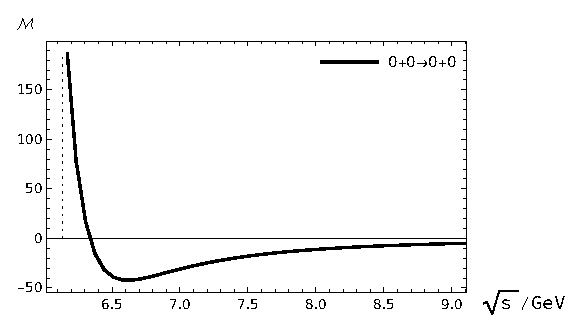
\includegraphics[width=0.49\textwidth]{../Others/1f.eps}
			% \caption{\small }
			\label{the1flavor}
			}\subfloat[Amplitudes for the contact term in $A(c\bar s)+B(c\bar s)\rightarrow C(c\bar s)+D(c\bar s)$.]{
			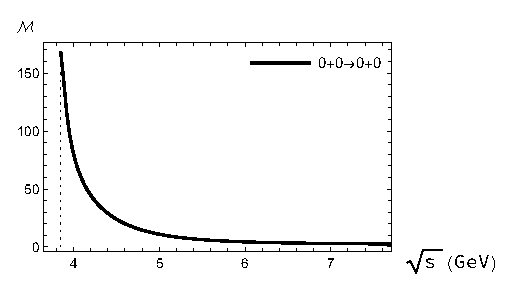
\includegraphics[width=0.49\textwidth]{../Others/2f.eps}
			% \caption{\small }
			\label{the1flavor}
			}\\ 
			
			\subfloat[Amplitudes for the contact term in $A(c\bar u)+B(c\bar d)\rightarrow C(c\bar u)+D(c\bar d)$.]{
			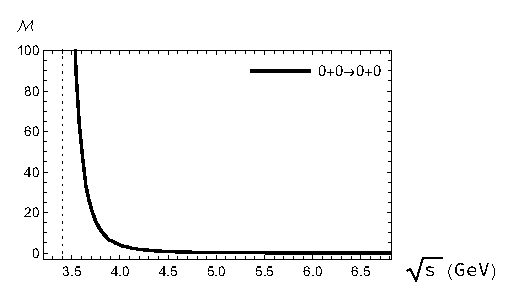
\includegraphics[width=0.49\textwidth]{../Others/3f.eps}
			% \caption{\small }
			\label{the1flavor}
			}
			\subfloat[Amplitudes for the contact term in $A(c\bar d)+B(b\bar s)\rightarrow C(b\bar d)+D(c\bar s)$ with particle B moving backwards. No near-threshold enhancement.]{
			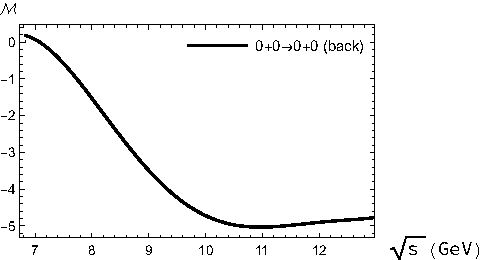
\includegraphics[width=0.49\textwidth]{../Others/4f.pdf}
			% \caption{\small }
			\label{the1flavor}
			}
	\end{figure}


\end{frame}

\section{NRQCD Factorization for Fully-heavy Tetraquark Production}
\begin{frame}
	\frametitle{Factorization theorem for $T_{4c/b}$ production}

	\begin{itemize}
		\begin{minipage}{0.4\textwidth}
			\item {\tt LHCb} discovered a narrow structure near $6.9$ GeV in the di-$J/\psi$ invariant mass spectrum ($>5\sigma$): $X(6900)$.
			\item Strong candidate for fully-charmed tetraquark.
		\end{minipage}\hfill
		\begin{minipage}{0.5\textwidth}
			\begin{figure}
				\centering
				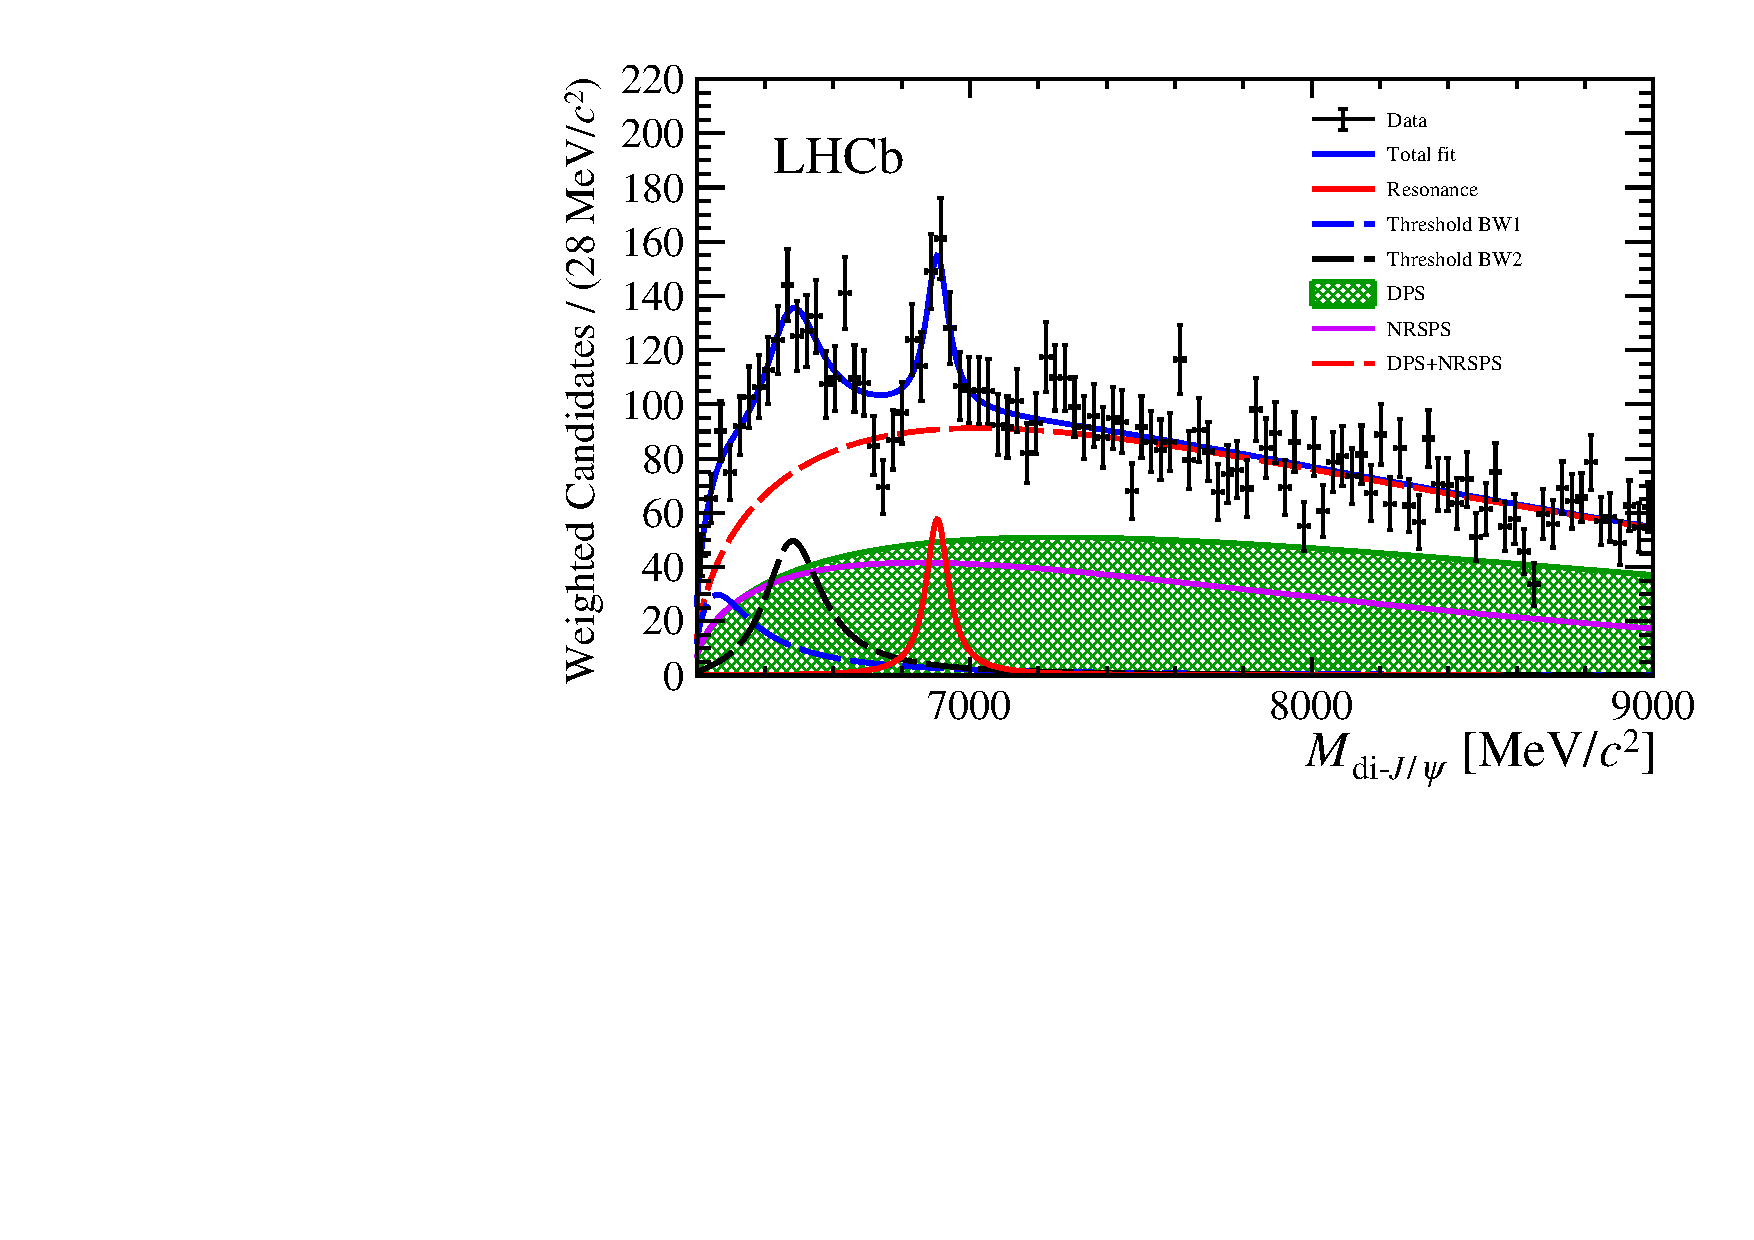
\includegraphics[width=\textwidth,frame]{../Others/Fig3b.pdf}
			\end{figure}
		\end{minipage}
		\item QCD factorization theorem for fully-heavy tetraquark ($T_{4c/b}$) exclusive production at high-$p_T$
		\begin{align}
			\mathrm{d} \sigma\left(p p \rightarrow T_{4c/b}\left(p_{\mathrm{T}}\right)+X\right) &=\sum_{i}\int_0^1 \mathrm{d} x_a  \int_0^1 \mathrm{d} x_b \int_{0}^{1} \mathrm{d} z\; f_{a/p}(x_a,\mu)f_{b/p}(x_b,\mu) \notag\\
			\times  \dd &{\hat \sigma}(a b \rightarrow i(p_T/z)+X, \mu)  D_{i \rightarrow T_{4c/b}}\left(z,\mu\right)+{\cal O}(1/p_T). 
			%-----------------------------------
			\label{QCD:fact:theor}
		\end{align}
		\item Dominate partonic channel is $gg\to gg$, rather than $gg\to q\bar{q}$. 
	\end{itemize}

\end{frame}

\begin{frame}
	\frametitle{Fragmentation Function}

	Collins-Soper definition of fragmentation function: 
	{\footnotesize
	\begin{align*}
		\begin{aligned}[b]
			&D_{g \rightarrow T_{4c}}(z, \mu)= \frac{-g_{\mu \nu} z^{d-3}}{2 \pi k^{+}\left(N_{c}^{2}-1\right)(d-2)} \int_{-\infty}^{+\infty} d x^{-} e^{-i k^{+} x^{-}}
			\\
			&\times\sum_X \left\langle 0\left|G_{c}^{+\mu}(0) \mathcal{E}^{\dagger}\left(0,0, \mathbf{0}_{\perp}\right)_{c b}
			|T_{4c}(P)+X\rangle\langle T_{4c}(P)+X| \mathcal{E}\left(0, x^{-}, \mathbf{0}_{\perp}\right)_{b a} G_{a}^{+\nu}\left(0, x^{-}, \mathbf{0}_{\perp}\right)\right| 0\right\rangle
		\end{aligned}
	\end{align*}}
	
	\begin{itemize}
		\item c/b quarks are heavy enough such that Fock states with light quarks or gluons are suppressed
		\item Similar to quarkonium cases
		\only<1>{\item NRQCD factorization for $T_{4c/b}$ production: 
		\begin{align}
			%-----------------------------------
			\notag D_{g \rightarrow T_{4 c}}\left(z, \mu_{\Lambda}\right) =
			&\frac{d_{3, 3}\left[g \rightarrow c c \bar{c} \bar{c}^{(J)}\right]}{m^{9}}\mel{0}{\mathscr{O}_{3,3}^{(J)}}{0}
			+\frac{d_{6,6}\left[g \rightarrow c c \bar{c} \bar{c}^{(J)}\right]}{m^{9}}\mel{0}{\mathscr{O}_{6,6}^{(J)}}{0}\\
			&+\frac{d_{3, 6}\left[g \rightarrow c c \bar{c} \bar{c}^{(J)}\right]}{m^{9}} 2{\rm Re}\left[\mel{0}{\mathscr{O}_{3,6}^{(J)}}{0}\right]
			+\cdots,
			%-----------------------------------
			\label{NRQCD:fac:Tc:fragmentation}
			%-----------------------------------
		\end{align}}
		\only<2>{\item Vacuum saturation approximation to suppress extra intermediate states
		\begin{align*}
			&\mathscr{O}^{(J)}_{3,3} = \mathcal{O}^{(J)}_{\mathbf{\bar 3}\otimes\mathbf{3}}\sum_X|T_{4c}^J+X\rangle\langle T_{4c}^J+X|\mathcal{O}^{(J)\dagger}_{\mathbf{\bar 3}\otimes\mathbf{3}}\\ 
			&\mathscr{O}^{(J)}_{6,6} = \mathcal{O}^{(J)}_{\mathbf{6}\otimes\bar{\mathbf{6}}}\sum_X|T_{4c}^J+X\rangle\langle T_{4c}^J+X|\mathcal{O}^{(J)\dagger}_{\mathbf{6}\otimes\bar{\mathbf{6}}}\\ 
			&\mathscr{O}^{(J)}_{3,6} = \mathcal{O}^{(J)}_{\mathbf{\bar 3}\otimes\mathbf{3}}\sum_X|T_{4c}^J+X\rangle\langle T_{4c}^J+X|\mathcal{O}^{(J)\dagger}_{\mathbf{6}\otimes\bar{\mathbf{6}}}
		\end{align*}}
	\end{itemize}
	% \begin{minipage}{0.49\textwidth}
	% 	{\small\begin{itemize}
	% 		\item NRQCD factorization: 
	% 		\begin{align*}
	% 			D_{g \rightarrow H}(z)=\sum_{n} d_{n}(z)\left\langle 0\left|\mathcal{O}_{n}^{H}\right| 0\right\rangle
	% 		\end{align*}
	% 		\item Perturbative matching to determine short distance coefficients. 
	% 		\item Use wave-function origin (S-wave) from potential models to determine long range matrix elements in order to yield a phenomenological result. 
	% 		\item More details in Jia-Yue Zhang's talk this afternoon. 
	% 	\end{itemize}}
	% \end{minipage}\hfill
	% \begin{minipage}{0.45\textwidth}
	% 	\begin{figure}[hbtp]
	% 		\centering
	% 		\begin{tikzpicture}[transform shape,scale=0.7]
	% 			\begin{feynman}
	% 				\node[crossed dot] (a);
	% 				\node[right=2.5in of a,crossed dot] (b);
	% 				\vertex at ($(a)+(0.3in,0.6in)$) (v1);
	% 				\vertex at ($(b)+(-0.3in,0.6in)$) (v2);
	% 				\vertex at ($(a)!0.5!(b)$) (o);
	% 				\vertex at ($(o)+(-0.2in,0.7in)$) (o1);
	% 				\vertex at ($(o)+(0.2in,0.7in)$) (o2);
	% 				\vertex at ($(o1)+(0in,1cm)$) (end1);
	% 				\vertex at ($(o1)+(0in,-1cm)$) (end2);
	% 				\vertex at ($(end1)!0.125!(end2)$) (f1);
	% 				\vertex at ($(end1)!0.375!(end2)$) (f2);
	% 				\vertex at ($(end1)!0.625!(end2)$) (f3);
	% 				\vertex at ($(end1)!0.875!(end2)$) (f4);
	% 				\vertex at ($(v1)!0.3!(f2)$) (i1);
	% 				\vertex at ($(i1)+(0.15in,-0.15in)$) (i2);
	% 				\vertex at ($(o2)+(0in,1cm)$) (end11);
	% 				\vertex at ($(o2)+(0in,-1cm)$) (end12);
	% 				\vertex at ($(end11)!0.125!(end12)$) (f11);
	% 				\vertex at ($(end11)!0.375!(end12)$) (f12);
	% 				\vertex at ($(end11)!0.625!(end12)$) (f13);
	% 				\vertex at ($(end11)!0.875!(end12)$) (f14);
	% 				\vertex at ($(v2)!0.3!(f12)$) (i11);
	% 				\vertex at ($(i11)+(-0.15in,-0.15in)$) (i12);
	% 				\vertex at ($(o)!0.66!(b)$) (t1);
	% 				\vertex at ($(i2)!0.33!(f4)$) (t2);
	% 				\vertex at ($(i12)!0.33!(f14)$) (t3);
	% 				\diagram*{
	% 					(v1) --[gluon,quarter right, looseness=0.7] (a);
	% 					(b) --[gluon,quarter right, looseness=0.7] (v2);
	% 					(v1) --[anti fermion, thick] (f1);
	% 					(v1) --[fermion, thick] (f2);
	% 					(i1) --[gluon] (i2);
	% 					(i2) --[fermion, thick] (f3);
	% 					(i2) --[anti fermion, thick] (f4);
	% 					(v2) --[anti fermion, thick] (f11);
	% 					(t1) --[gluon,quarter right, looseness=0.7] (i12);
	% 					(v2) --[fermion, thick] (f12);
	% 					(i12) --[fermion, thick] (f13);
	% 					(i12) --[anti fermion, thick] (f14);
	% 					(t2) --[gluon,half right, looseness=1.2] (t3);
	% 					(a) --[double distance=2pt] (b);
	% 				};
	% 				\draw[fill=gray!30!white] (o1) ellipse (0.2cm and 1cm);
	% 				\draw[fill=gray!30!white] (o2) ellipse (0.2cm and 1cm);
	% 				\vertex at ($(o)+(0in,-0.3in)$) (cut1);
	% 				\vertex at ($(o)+(0in,1.2in)$) (cut2);
	% 				\vertex at ($(cut2)+(0.2in,0.2in)$) (cut11);
	% 				\vertex at ($(cut1)+(-0.2in,-0.2in)$) (cut22);
	% 				\draw[dashed] (cut1) -- (cut2);
	% 				\draw[dashed] (cut2) to[out=90,in=180] (cut11);
	% 				\draw[dashed] (cut1) to[out=270,in=0] (cut22);
	% 			\end{feynman}
	% 		\end{tikzpicture}
	% 		\caption{A representative Feynman diagram for the fragmentation function of gluon into $T_{4c}$. The grey blob indicates
	% 		the $C$-even tetraquark. Horizontal double line denotes the eikonal line.}
	% 		\label{tetra-diagrams}
	% 	\end{figure}
	% \end{minipage}

\end{frame}

\begin{frame}
	\frametitle{Fragmentation Function}

	
	\begin{itemize}
		\item Local tetraquark operators:
		\begin{subequations}
			%-----------------------------------
			\begin{align}
			%-----------------------------------
			 &\mathcal{O}^{(0)}_{\mathbf{\bar 3}\otimes\mathbf{3}}=-\frac{1}{\sqrt{3}}[\psi_a^T(i\sigma^2)\sigma^i\psi_b] [\chi_c^{\dagger}\sigma^i (i\sigma^2)\chi_d^*]\;
			 \mathcal{C}^{ab;cd}_{\mathbf{3}\otimes\bar{\mathbf{3}}},
			%-----------------------------------
			\\
			%-----------------------------------
			 &\mathcal{O}^{\alpha\beta;(2)}_{\mathbf{\bar 3}\otimes\mathbf{3}} =[\psi_a^T(i\sigma^2)\sigma^m\psi_b] [\chi_c^{\dagger}\sigma^n(i\sigma^2)\chi_d^*]\;{\Gamma^{\alpha\beta;mn}}
			 \;\mathcal{C}^{ab;cd}_{\mathbf{3}\otimes\bar{\mathbf{3}}},
			%-----------------------------------
			\\
			%-----------------------------------
			&{\mathcal{O}^{(0)}_{\mathbf{6}\otimes\bar{\mathbf{6}}} =
			[\psi_a^T(i\sigma^2)\psi_b] [\chi_c^{\dagger}(i\sigma^2)\chi_d^*]\;
			\mathcal{C}^{ab;cd}_{\mathbf{6}\otimes\bar{\mathbf{6}}}},
			%-----------------------------------
			\end{align}
			%-----------------------------------
			\label{NRQCD:composite:operators}
			%-----------------------------------
		\end{subequations}
		The rank-4 Lorentz tensor is given by $\Gamma^{\alpha\beta;mn}\equiv {\frac{1}{2}}[g^{\alpha m} g^{\beta n}+g^{\alpha n} g^{\beta m}-\frac{1}{2} g^{\alpha \beta} g^{mn}]$,
		and the rank-4 color tensors read
		%-----------------------------------
		\begin{subequations}
		%-----------------------------------
		\begin{align}
		%-----------------------------------
		& {\mathcal{C}^{ab;cd}_{\mathbf{3} \otimes\bar{\mathbf{3}}}\equiv \frac{1}{(\sqrt{2})^2} \epsilon^{abm}\epsilon^{cdn}\frac{\delta^{mn}}{\sqrt{N_c}}=\frac{1}{2\sqrt{3}}(\delta^{ac}\delta^{bd}-\delta^{ad}\delta^{bc})}
		%-----------------------------------
		\\
		%-----------------------------------
		& \mathcal{C}^{ab;cd}_{\bar{\mathbf{6}}\otimes\mathbf{6}}
		\equiv \frac{1}{2\sqrt{6}}(\delta^{ac}\delta^{bd}+\delta^{ad}\delta^{bc}).
		%-----------------------------------
		\end{align}
		%-----------------------------------
		\label{color:tensor}
		%-----------------------------------
		\end{subequations}
	\end{itemize}
\end{frame}

\begin{frame}
	\frametitle{Fragmentation Function}

	\begin{minipage}{0.49\textwidth}
		{\small\begin{itemize}
			\item NRQCD factorization: 
			\begin{align*}
				D_{g \rightarrow H}(z)=\sum_{n} d_{n}(z)\left\langle 0\left|\mathcal{O}_{n}^{H}\right| 0\right\rangle
			\end{align*}
			\item Perturbative matching to determine short distance coefficients. 
			\item Use wave-function origin (S-wave) from potential models to determine long range matrix elements in order to yield a phenomenological result. 
			\item More details in Jia-Yue Zhang's talk this afternoon. 
		\end{itemize}}
	\end{minipage}\hfill
	\begin{minipage}{0.45\textwidth}
		\begin{figure}[hbtp]
			\centering
			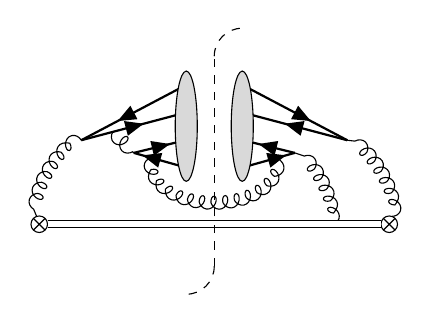
\begin{tikzpicture}[transform shape,scale=0.7]
				\begin{feynman}
					\node[crossed dot] (a);
					\node[right=2.5in of a,crossed dot] (b);
					\vertex at ($(a)+(0.3in,0.6in)$) (v1);
					\vertex at ($(b)+(-0.3in,0.6in)$) (v2);
					\vertex at ($(a)!0.5!(b)$) (o);
					\vertex at ($(o)+(-0.2in,0.7in)$) (o1);
					\vertex at ($(o)+(0.2in,0.7in)$) (o2);
					\vertex at ($(o1)+(0in,1cm)$) (end1);
					\vertex at ($(o1)+(0in,-1cm)$) (end2);
					\vertex at ($(end1)!0.125!(end2)$) (f1);
					\vertex at ($(end1)!0.375!(end2)$) (f2);
					\vertex at ($(end1)!0.625!(end2)$) (f3);
					\vertex at ($(end1)!0.875!(end2)$) (f4);
					\vertex at ($(v1)!0.3!(f2)$) (i1);
					\vertex at ($(i1)+(0.15in,-0.15in)$) (i2);
					\vertex at ($(o2)+(0in,1cm)$) (end11);
					\vertex at ($(o2)+(0in,-1cm)$) (end12);
					\vertex at ($(end11)!0.125!(end12)$) (f11);
					\vertex at ($(end11)!0.375!(end12)$) (f12);
					\vertex at ($(end11)!0.625!(end12)$) (f13);
					\vertex at ($(end11)!0.875!(end12)$) (f14);
					\vertex at ($(v2)!0.3!(f12)$) (i11);
					\vertex at ($(i11)+(-0.15in,-0.15in)$) (i12);
					\vertex at ($(o)!0.66!(b)$) (t1);
					\vertex at ($(i2)!0.33!(f4)$) (t2);
					\vertex at ($(i12)!0.33!(f14)$) (t3);
					\diagram*{
						(v1) --[gluon,quarter right, looseness=0.7] (a);
						(b) --[gluon,quarter right, looseness=0.7] (v2);
						(v1) --[anti fermion, thick] (f1);
						(v1) --[fermion, thick] (f2);
						(i1) --[gluon] (i2);
						(i2) --[fermion, thick] (f3);
						(i2) --[anti fermion, thick] (f4);
						(v2) --[anti fermion, thick] (f11);
						(t1) --[gluon,quarter right, looseness=0.7] (i12);
						(v2) --[fermion, thick] (f12);
						(i12) --[fermion, thick] (f13);
						(i12) --[anti fermion, thick] (f14);
						(t2) --[gluon,half right, looseness=1.2] (t3);
						(a) --[double distance=2pt] (b);
					};
					\draw[fill=gray!30!white] (o1) ellipse (0.2cm and 1cm);
					\draw[fill=gray!30!white] (o2) ellipse (0.2cm and 1cm);
					\vertex at ($(o)+(0in,-0.3in)$) (cut1);
					\vertex at ($(o)+(0in,1.2in)$) (cut2);
					\vertex at ($(cut2)+(0.2in,0.2in)$) (cut11);
					\vertex at ($(cut1)+(-0.2in,-0.2in)$) (cut22);
					\draw[dashed] (cut1) -- (cut2);
					\draw[dashed] (cut2) to[out=90,in=180] (cut11);
					\draw[dashed] (cut1) to[out=270,in=0] (cut22);
				\end{feynman}
			\end{tikzpicture}
			\caption{A representative Feynman diagram for the fragmentation function of gluon into $T_{4c}$. The grey blob indicates
			the $C$-even tetraquark. Horizontal double line denotes the eikonal line.}
			\label{tetra-diagrams}
		\end{figure}
	\end{minipage}

\end{frame}

\begin{frame}
	\frametitle{Phenomenology for $T_{4c/b}$ production at LHC}

	% \begin{minipage}{0.24\textwidth}
	% 	\begin{itemize}
	% 		\item 
	% 	\end{itemize}
	% \end{minipage}
	\begin{minipage}{0.99\textwidth}
		\begin{figure}[!hbtp]
			\centering
			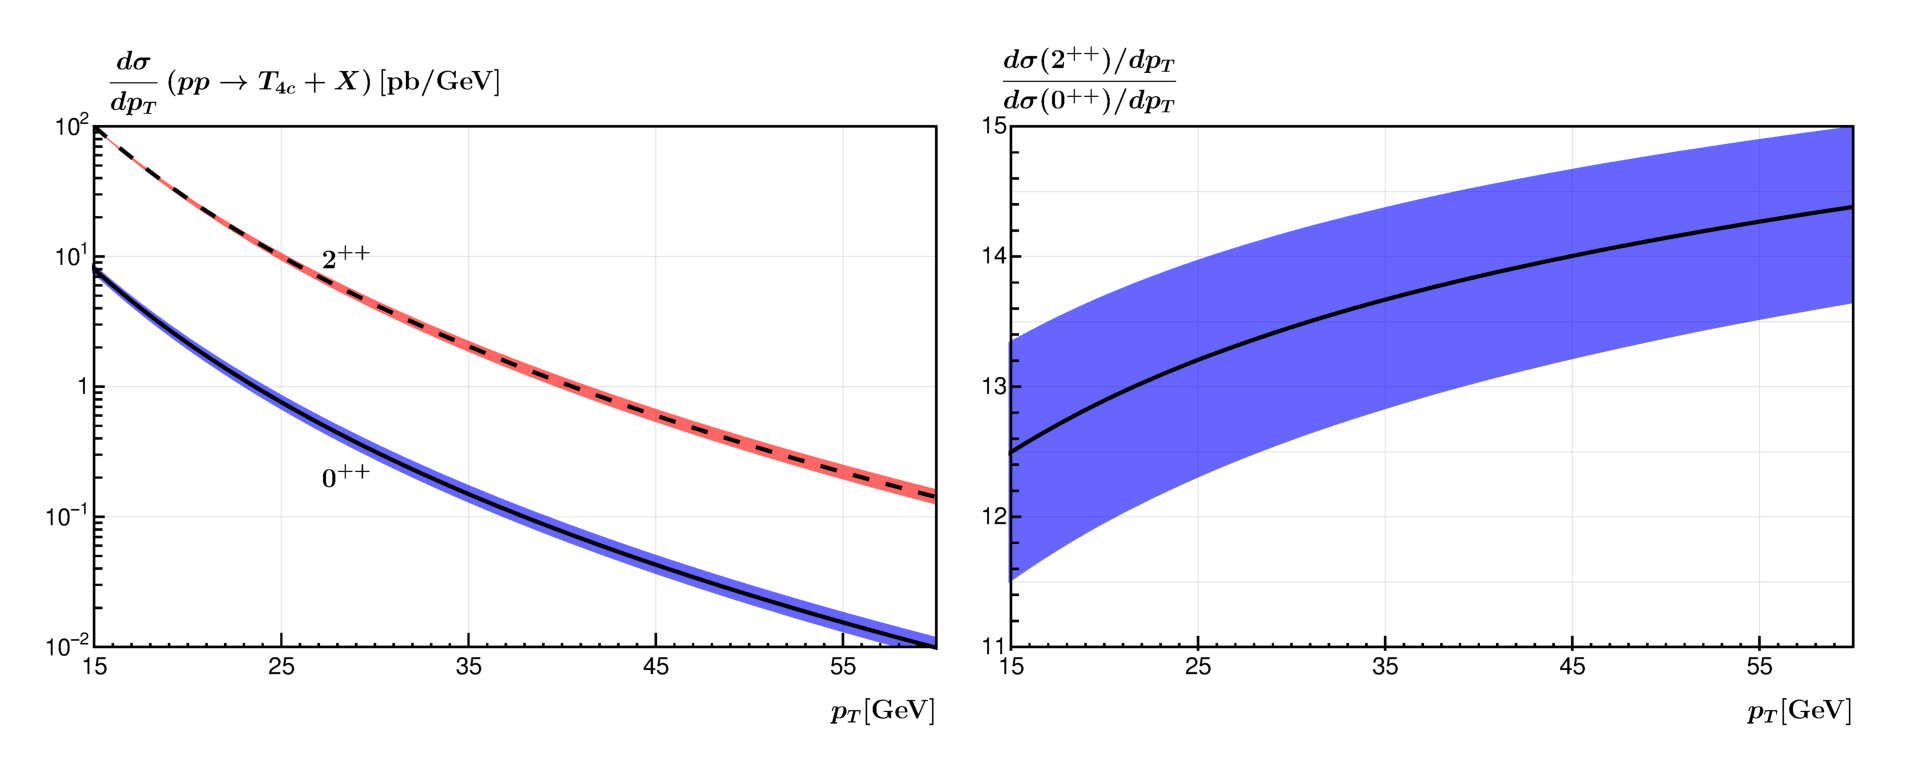
\includegraphics[width=\textwidth,frame]{../Others/cpTFig.eps}
			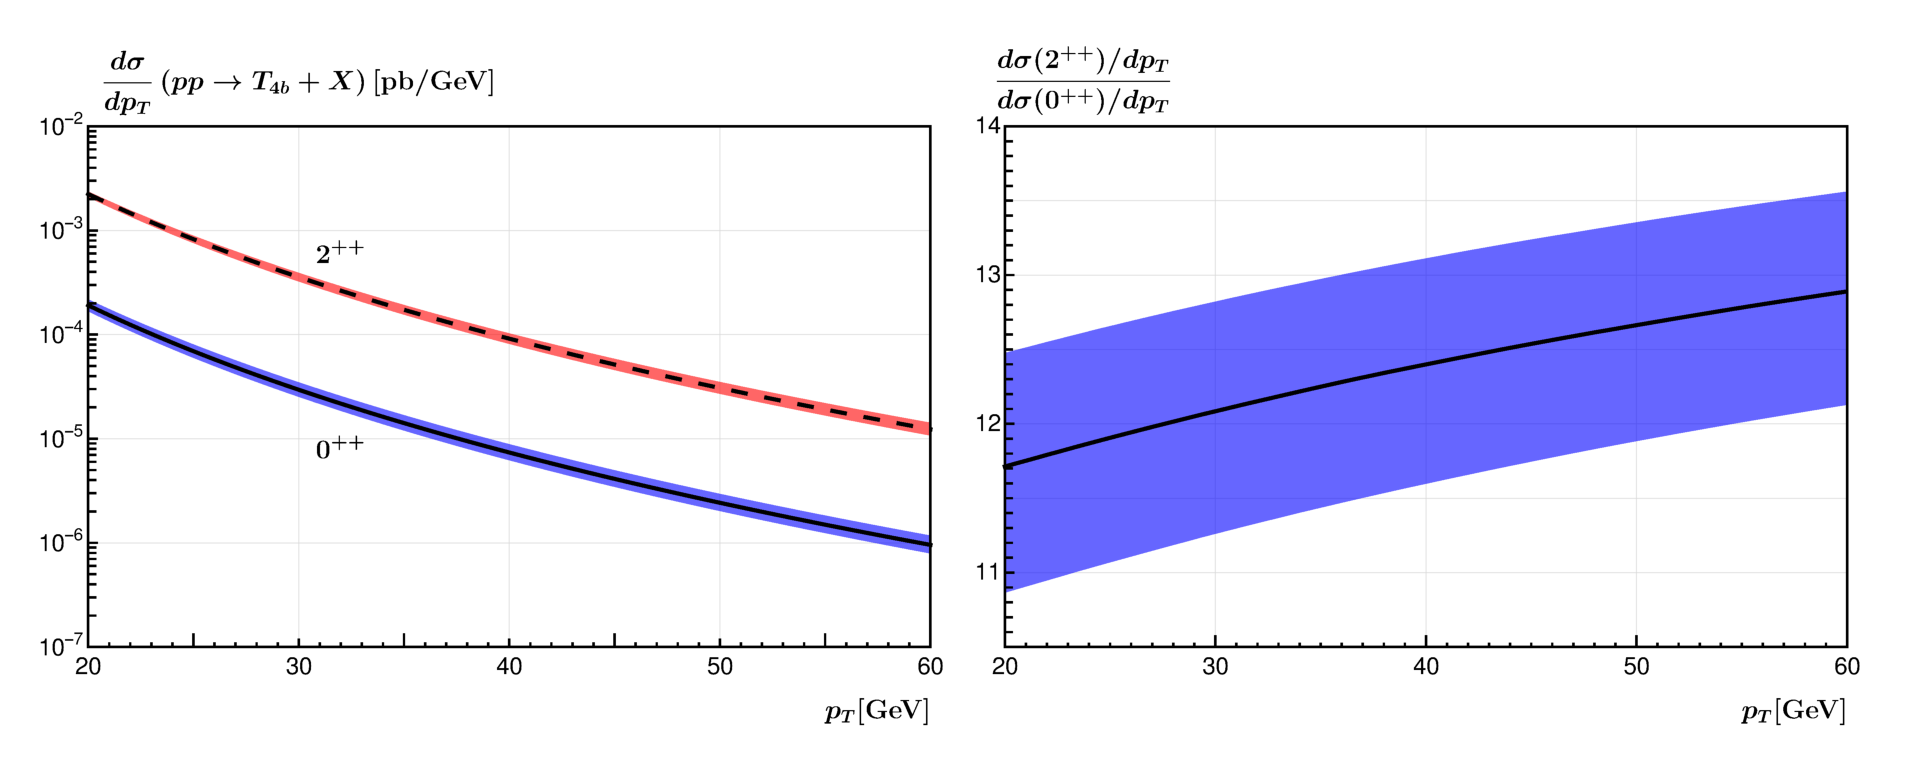
\includegraphics[width=\textwidth,frame]{../Others/bpTFig.eps}
			% \caption{The $p_T$ distribution of inclusive $T_{4c/4b}$ production on LHC. The central values (represented by the solid and dashed curves) are generated by setting $\mu=p_T$. The difference between $0^{++}$ and $2^{++}$ states are also given. }
			\label{fig:pT_dstrbtn}
		\end{figure}
	\end{minipage}

\end{frame}

\begin{frame}
	\frametitle{Phenomenology for $T_{4c/b}$ production at LHC}

	\begin{itemize}
		\item $2^{++}$ cross section is about 10 times larger than $0^{++}$. 
		\item We obtain the yields of the accumulated event number for $T_{4c}$ at HL-LHC are a hundred million for $0^{++}$ and 8 hundreds million for $2^{++}$ (with integrated luminosity 3000 $\rm{fb}^{-1}$). 
		\item The
		prediction for $T_{4b}$ is highly suppressed, mainly due to the relative larger bottom mass suppression.
		\item The total cross section we obtained is unreliable mainly due to the fact that fragmentation only works at high-$p_T$, and our integration is done within approximately $15\leq p_T\leq 60 \rm{GeV}$.
		% \begin{table}[h]
		% 	{\small\begin{tabular}{|c|c|c|c|c|c|}
		% 		\hline
		% 		&  & \multicolumn{2}{c|}{$0^{++}$} & \multicolumn{2}{c|}{$2^{++}$ }\tabularnewline
		% 		\hline
		% 		& $p_{T}$ range & $\sigma$  & $N_{\mathrm{events}}$ & $\sigma$  & $N_{\mathrm{events}}$\tabularnewline
		% 		\hline
		% 		$T_{4c}$ & $15\mathrm{\mathrm{GeV}}\leq p_{T}\leq60\mathrm{\mathrm{GeV}}$  & $33_{-4}^{+4}\mathrm{pb}$ & $9.9_{-1.2}^{+1.2}\times10^{7}$ & $424_{-21}^{+13}\mathrm{pb}$ & $1.27_{-0.06}^{+0.04}\times10^{9}$\tabularnewline
		% 		\hline
		% 		$T_{4b}$ & $20\mathrm{\mathrm{GeV}}\leq p_{T}\leq60\mathrm{\mathrm{GeV}}$  & $1.04_{-0.15}^{+0.17}\times10^{-3}\mathrm{pb}$ & $3.12_{-0.45}^{+0.51}\times10^{3}$ & $1.24_{-0.11}^{+0.11}\times10^{-2}\mathrm{pb}$ & $3.72_{-0.33}^{+0.33}\times10^{4}$\tabularnewline
		% 	\hline
		% 	\end{tabular}}
		% \caption{The $p_T$-integrated cross section for $T_4c$ inclusive production on LHC.}
		% \label{pT_intgrtd}
		% \end{table}
	\end{itemize}

\end{frame}

\begin{frame}
  \frametitle{Summary \& Outlook}
  {\bf Summary: }
  \begin{itemize}
    \item Production mechanism for fully-heavy tetraquark $T_{4c/b}$ hasn't been well discussed on a QCD basis
    \item We propose a framework for $T_{4c/b}$ production based on NRQCD factorization
    \item We adopt fragmentation mechanism for $T_{4c/b}$ production @LHC
    \item Calculate FF from QCD-based Collins-Soper definition, FF is factorized into SDCs and NRQCD LDMEs
    \item Defined LO NRQCD local operators and derived LO SDCs for $D_{g \rightarrow T_{4c}}$
    \item We use phenomenological wave functions at origin to obtain predictions of cross sections
  \end{itemize}
  {\bf Outlook: }
  \begin{itemize}
    \item Production at other experiments
    \item P-wave $T_{4c/b}$
  \end{itemize}

\end{frame}

\begin{frame}
	\frametitle{Research Plans}
	\Large
	\begin{itemize}
		\item New projects: 
		Anything QCD or EFT related
		\item Old projects: 
		\begin{itemize}
			\item Three body OPE to the 1st order 
			\item Fully reconstruct Schroedinger wave function with OPE (renormalization problem for QM)
			\item P-wave tetraquark fragmentation function 
			\item Top loop Coulomb resummation
		\end{itemize}
	\end{itemize}

\end{frame}



\appendix
\begin{frame}[standout]
  \Huge Questions?
\end{frame}
% \begin{frame}
% 	\begin{center}
% 		\Huge 
% 		\usebeamercolor[bg]{frametitle}
% 		\emph{Thanks for your attention!}
% 	\end{center}
% \end{frame}

\appendix
\begin{frame}
  \vfill
  \centering
  \begin{beamercolorbox}[sep=8pt,center,shadow=true,rounded=true]{title}
    \usebeamerfont{title}Backup\par%
  \end{beamercolorbox}
  \vfill
\end{frame}

\begin{frame}
  \frametitle{bottom versus charm}

  \begin{itemize}
    \item Charm:
          \begin{align*}
            \alpha_s(4m_c)=0.22,\; m_c=1.5 \rm{GeV},\; R_{D_c}(0)=0.523\;\mathrm{GeV}^{3/2},\;R_{T_c}(0)=2.902 \;\mathrm{GeV}^{3/2}
          \end{align*}
    \item Bottom:
          \begin{align*}
            \alpha_s(4m_b)=0.17,\; m_b=4.8 \rm{GeV},\; R_{D_b}(0)=0.703\;\mathrm{GeV}^{3/2},\;R_{T_b}(0)=5.579 \;\mathrm{GeV}^{3/2}
          \end{align*}
    \item The ratio is
          \begin{align*}
                    & \pqty{\frac{\alpha_s(4m_c)}{\alpha_s(4m_b)}}^4\pqty{\frac{ m_c}{ m_b}}^{-9}\pqty{\frac{R_{T_c}(0)}{R_{T_b}(0)}}^2\pqty{\frac{R_{D_c}(0)}{R_{D_b}(0)}}^4 \\
            =       & {\left(\frac{0.22}{0.17}\right)^4\left(\frac{1.5}{4.8}\right)^{-9} \left(\frac{2.902}{5.579}\right)^2 \left(\frac{0.523}{0.703}\right)^4}               \\
            \approx & 10^4
          \end{align*}
  \end{itemize}

\end{frame}

\printbibliography

% \bibliography{../Bib}
% \bibliographystyle{apalike}

\end{document}
